\pdfcompresslevel=1
\pdfobjcompresslevel=1
\documentclass[12pt,a4paper]{report}

% ---------- Encoding & Language ----------
\usepackage[utf8]{inputenc}
\usepackage[T1]{fontenc}
\usepackage{lmodern}
\usepackage[english]{babel}

% ---------- Page Geometry & Spacing ----------
\usepackage{geometry}
\geometry{margin=1in}
\usepackage{setspace}
\onehalfspacing

% ---------- Figures, Tables, Math ----------
\usepackage{graphicx}
\usepackage{xcolor}
\usepackage{booktabs}
\usepackage{tabularx}
\usepackage{longtable}
\usepackage{multirow}
\usepackage{float}
\usepackage{amsmath, amssymb}
\usepackage{array}
\usepackage{enumitem}
\usepackage{ragged2e}
\usepackage{algorithm}
\usepackage{algpseudocode}

\setlist{leftmargin=2em}
\setlist[itemize]{nosep,leftmargin=2em}
\newcolumntype{R}[1]{>{\RaggedLeft\arraybackslash}p{#1}}
\newcolumntype{L}[1]{>{\RaggedRight\arraybackslash}p{#1}}
\setlength{\arrayrulewidth}{0.4pt}
\renewcommand{\arraystretch}{1.12}

% ---------- Hyperlinks ----------
\usepackage{hyperref}
\hypersetup{
    colorlinks=true,
    linkcolor=blue,
    citecolor=blue,
    urlcolor=blue,
    pdfauthor={Nguyen Van Thanh, Nguyen Chien Thang, Nguyen Hoang Tuyen, Le Thanh Phuong},
    pdftitle={Real-Time Passive Face Anti-Spoofing Using Aligned Lightweight Convolutional Networks for Biometric Attendance Verification},
}

% ---------- Typography & Hyphenation ----------
\usepackage[protrusion=true,expansion=false]{microtype}
\usepackage[none]{hyphenat}
\sloppy
\emergencystretch=2em

% ---------- Title Page Frame ----------
\usepackage{tikz}
\newcommand{\pageframe}{%
  \begin{tikzpicture}[remember picture,overlay]
    \draw[line width=0.8pt]
      ([xshift=1cm,yshift=-1cm]current page.north west)
      rectangle
      ([xshift=-1cm,yshift=1cm]current page.south east);
  \end{tikzpicture}%
  \begin{tikzpicture}[remember picture,overlay]
    \draw[line width=0.8pt]
      ([xshift=1.1cm,yshift=-1.1cm]current page.north west)
      rectangle
      ([xshift=-1.1cm,yshift=1.1cm]current page.south east);
  \end{tikzpicture}%
}

\begin{document}

\begin{titlepage}
    \pageframe 
    \begin{center}
        \vspace*{-1cm} 
        
        % FPTU Logo
        \includegraphics[width=0.6\linewidth]{Images/FPT University logo.png}

        \vspace*{0.5cm}
        
        % Adjusted title size to fit cleanly on one page
        \Large
        \textbf{REAL-TIME PASSIVE FACE ANTI-SPOOFING USING ALIGNED LIGHTWEIGHT CONVOLUTIONAL NETWORKS FOR BIOMETRIC ATTENDANCE VERIFICATION}
 
        \vspace{0.3cm}
        \vfill
        \begin{table}[H]
        \large
        \centering
        \begin{tabular}{rl}
        Team members: & HE181962 - Nguyen Van Thanh \\
                      & HE186312 - Nguyen Chien Thang \\
                      & HE180882 - Nguyen Hoang Tuyen \\
                      & HE186753 - Le Thanh Phuong \\
                      &                           \\
        Supervisor:   & MSc. Nguyen Ngoc Huy      
        \end{tabular}
        \end{table}
        \Large

        \vspace{0.25cm}
        \vfill
        \Large
        Bachelor of Artificial Intelligence\\
        FPT University - Oct 2026\\
    \end{center}
\end{titlepage}

\chapter*{Acknowledgements}
\addcontentsline{toc}{chapter}{Acknowledgements}

First and foremost, the project team expresses sincere gratitude to the thesis supervisor, MSc. Nguyen Ngoc Huy, for his patient mentorship, rigorous technical feedback, and thoughtful direction throughout every stage of this capstone work. His insistence on empirical verification, clean dataset boundaries, and practical engineering standards shaped both the methodology and the experimental evaluation presented in this thesis.

Appreciation is also extended to the faculty members of the Department of Artificial Intelligence at FPT University, Hoa Lac Campus, whose coursework in computer vision, deep learning, and software engineering established the foundation required to design, debug, and deploy an end-to-end biometric security system. Special thanks are owed to the fellow students and volunteers who consented to participate in multi-session video acquisition for presentation attack testing.

Finally, the team members thank their families for their steady encouragement, patience, and support throughout the undergraduate program.

\chapter*{Abstract}
\addcontentsline{toc}{chapter}{Abstract}
\normalsize

Automated facial attendance and access control systems deployed on standard monocular RGB cameras remain vulnerable to presentation attacks, particularly video replays on mobile screens and printed photographs that impersonate enrolled users without specialized depth or infrared sensors. To close this security gap on commodity CPU hardware, this thesis develops a real-time passive face anti-spoofing framework built around a compact $545{,}154$-parameter convolutional neural network (\texttt{LivenessNet}) operating on $32 \times 32$ local facial patches, paired with OpenCV YuNet detection, video-balanced training queues, weight-space interpolation, and a frozen TensorFlow Lite XNNPACK execution runtime. Methodological investigation progressed across two complementary datasets: a multi-source corpus of $28{,}957$ facial crops from $89$ videos used to diagnose normalization drift under imbalanced domain merging, and a dedicated subject-disjoint benchmark of $26{,}094$ facial crops extracted from $91$ 4K recordings on a USB SC-M200 camera. Controlled ablation experiments revealed that replacing Batch Normalization with Group and Layer Normalization alongside stratified $4 \times 8$ source-class-video mini-batches reduced the Attack Presentation Classification Error Rate from $16.16\%$ to $4.44\%$ on the merged benchmark. Subsequent feature-aligned adaptation on the SC-M200 corpus achieved $98.88\%$ validation frame accuracy, $98.09\%$ independent test frame accuracy ($1.94\%$ Average Classification Error Rate, with $99.88\%$ bona fide recall and $99.87\%$ spoof precision), $100.00\%$ video-level classification accuracy across all $14$ unseen test videos, and $99.84\%$ external cross-camera accuracy. Exported to unquantized LiteRT format, the classifier executes in $0.163$~ms median CPU latency, sustaining $30$ frames per second in a multi-threaded camera runtime, $40.61$~ms end-to-end HTTP microservice latency, and reliable spoof blocking within an InsightFace ArcFace web attendance application. These findings confirm that disciplined data partitioning, balanced optimization, and lightweight graph compilation enable practical passive liveness verification on standard office hardware.

\vspace{0.5cm}
\noindent\textbf{Keywords:} Face Anti-Spoofing; Presentation Attack Detection; Lightweight Convolutional Neural Network; Domain Generalization; Biometric Attendance System.


\tableofcontents
\listoffigures
\listoftables
\clearpage

\chapter{Introduction}
\label{chap:introduction}

\section{Background and Motivation}
\label{sec:background_motivation}

Contactless facial recognition has become a standard authentication mechanism across enterprise access control, university attendance tracking, and self-service check-in terminals. Modern deep metric-learning models, particularly additive angular margin architectures such as ArcFace~\cite{deng2019arcface}, achieve high verification accuracy on unconstrained monocular RGB images captured by commodity webcams. Despite strong identity discrimination, standard face recognition pipelines optimize solely for inter-class identity separation and remain inherently blind to physical liveness. When an unprotected attendance terminal observes a photograph printed on paper or a high-resolution portrait video replayed on a smartphone screen, the extracted facial embedding closely matches the enrolled template of the legitimate user, allowing unauthorized check-ins without specialized equipment~\cite{anjos2011counter, yu2023deep}.

In biometric security terminology standardized by ISO/IEC 30107-3~\cite{iso30107_3}, deliberate attempts to subvert a biometric capture sensor using physical artifacts are classified as presentation attacks, and the artifacts themselves---such as printed sheets, mobile displays, or three-dimensional masks---are termed Presentation Attack Instruments (PAIs). Presentation Attack Detection (PAD), commonly referred to as face anti-spoofing or liveness detection, acts as a security gate positioned upstream of or in parallel with identity matching. Commercial deployments in banking kiosks and flagship smartphones frequently rely on specialized multi-spectral sensors, including near-infrared (NIR) illuminators, structured-light depth projectors, or time-of-flight cameras~\cite{george2020biometric}. While active depth and thermal sensors simplify the separation of planar displays from three-dimensional facial geometry, their hardware cost, calibration requirements, and driver constraints prohibit widespread adoption in budget-constrained classrooms, small-to-medium offices, and browser-based attendance portals that operate exclusively on standard USB or integrated laptop RGB cameras.

Passive monocular RGB face anti-spoofing offers a hardware-agnostic alternative by inferring liveness directly from a conventional video stream without requiring user cooperation (such as prompted blinking or head-turn challenges, which slow throughput at busy entry points and remain vulnerable to pre-recorded video replay). Designing a reliable passive RGB PAD subsystem for real-time attendance verification nevertheless introduces three practical engineering tensions:
\begin{enumerate}
    \item \textbf{Sensor and domain sensitivity:} Subtle optical cues that distinguish live skin from electronic displays---such as subpixel moir\'{e} patterns, specular glass reflections, color gamut compression, and defocus blur---shift substantially across camera sensors, video compression containers, and indoor lighting conditions~\cite{wen2015face, jia2020single}.
    \item \textbf{Strict CPU latency budgets:} Edge attendance terminals routinely lack discrete graphics processing units (GPUs). Running face detection, identity embedding extraction, and anti-spoofing concurrently on a host CPU requires the PAD network to execute in sub-millisecond to low-millisecond budgets so that live video feedback remains responsive at $30$~frames per second (FPS).
    \item \textbf{Temporal decision stability:} Frame-by-frame softmax thresholding produces erratic visual flickering when a subject moves momentarily through overhead glare or motion blur, degrading user usability in interactive check-in kiosks and risking transient false acceptances in automated APIs.
\end{enumerate}

Motivated by these operational constraints, this thesis investigates, designs, and validates an end-to-end passive RGB face anti-spoofing framework built around an aligned lightweight convolutional network (\texttt{LivenessNet}), multi-source normalization and sampling diagnostics, low-latency LiteRT CPU execution, and fail-closed integration into a real-time WebSocket biometric attendance application.

\section{Literature Review}
\label{sec:literature_review}

Research on monocular RGB face presentation attack detection has progressed from handcrafted micro-texture descriptors to specialized deep convolutional architectures and cross-domain training paradigms. It should be noted that the objective of this subsection is to establish the practical necessity and research positioning of the present study rather than to examine mathematical formulations in full detail; a rigorous architectural and algorithmic analysis is deferred to Section~\ref{sec:exist_frameworks_algorithms} (\emph{Existing Frameworks and Algorithms}).

Early passive anti-spoofing studies observed that recapturing a face through a print medium or liquid-crystal display alters local spatial frequencies and color distributions. Chingovska et al.~\cite{chingovska2012effectiveness} established Local Binary Patterns (LBP) on the Replay-Attack benchmark~\cite{anjos2011counter}, while Zhang et al.~\cite{zhang2012face} introduced multi-scale DoG filtering on CASIA-FASD to isolate high-frequency screen noise and loss of facial edge sharpness. Wen et al.~\cite{wen2015face} formalized Image Distortion Analysis (IDA) using specular reflection, blurriness, chromatic moment, and color diversity features, and Boulkenafet et al.~\cite{boulkenafet2016face} demonstrated that extracting texture descriptors in luminance-chrominance spaces ($YC_bC_r$ and HSV) substantially outperforms grayscale analysis. Although computationally inexpensive on CPUs, handcrafted descriptors exhibit brittle thresholds when camera Automatic White Balance (AWB) or sensor resolution changes, as later documented on mobile benchmarks such as OULU-NPU~\cite{boulkenafet2017oulu}.

To overcome manual feature design, deep learning methods trained convolutional neural networks (CNNs) directly on facial crops or auxiliary supervisory signals. Liu et al.~\cite{liu2018learning} supervised a CNN-RNN architecture using pseudo-depth maps and remote photoplethysmography (rPPG) pulse signals, steering the network away from subject identity features toward geometric cues. Yu et al.~\cite{yu2020searching} introduced Central Difference Convolution Networks (CDCN) to combine intensity-level semantics with gradient-level micro-texture differentials. Large-scale benchmarks such as CelebA-Spoof~\cite{zhang2020celeba} enabled deeper backbones, whereas Wang et al.~\cite{wang2022patchnet} proposed PatchNet, showing that formulating anti-spoofing as fine-grained local patch recognition prevents global identity memorization and improves sensitivity to surface material properties. Concurrently, domain generalization studies such as Single-Side Domain Generalization (SSDG)~\cite{jia2020single} highlighted that naive pooling of heterogeneous datasets still suffers from covariate shift unless feature normalization is carefully controlled.

\begin{table}[htbp]
\centering
\caption{Summary of representative passive RGB face anti-spoofing paradigms and deployment trade-offs.}
\label{tab:lit_summary}
\small
\begin{tabular}{L{3.1cm}L{3.2cm}L{3.8cm}L{4.0cm}}
\toprule
\textbf{Paradigm} & \textbf{Representative Works} & \textbf{Primary Strengths} & \textbf{Deployment Limitations} \\
\midrule
Handcrafted Color \& Texture & LBP~\cite{chingovska2012effectiveness}, IDA~\cite{wen2015face}, Colour-LBP~\cite{boulkenafet2016face} & Low CPU cost; interpretable optical priors; minimal training data required. & Sensitive to AWB shifts, high-PPI OLED screens, and illumination variance. \\
\addlinespace[3pt]
Auxiliary Depth \& Physiological CNNs & Auxiliary Depth + rPPG~\cite{liu2018learning}, CDCN~\cite{yu2020searching} & Strong separation of planar vs.\ 3D live faces; reduced identity overfitting. & Multi-megabyte dense feature maps; elevated CPU latency without GPU acceleration. \\
\addlinespace[3pt]
Domain-Generalized \& Multi-Channel PAD & MCCNN~\cite{george2020biometric}, SSDG~\cite{jia2020single}, Survey~\cite{yu2023deep} & Improved cross-sensor transfer across heterogeneous acquisition domains. & Requires multi-domain adversarial/triplet training or auxiliary IR channels. \\
\addlinespace[3pt]
Local Patch \& Lightweight CNNs & PatchNet~\cite{wang2022patchnet}, MobileNetV3~\cite{howard2019searching} & Suppresses global identity cues; compact memory footprint suitable for edge CPUs. & Single-frame predictions flicker under motion/glare; vulnerable to BatchNorm drift under imbalanced merges. \\
\bottomrule
\end{tabular}
\end{table}

Table~\ref{tab:lit_summary} synthesizes these four research directions. A clear operational gap persists between academic benchmark models and deployable CPU attendance systems: methods with strong anti-spoofing accuracy frequently rely on heavy multi-branch architectures evaluated offline on isolated frames, whereas lightweight CNNs often suffer from evaluation leakage (frame-level random splits from identical videos), normalization miscalibration when combining uneven video cohorts, and unstable single-frame decision logic during live camera streaming.

\section{Problem Statement}
\label{sec:problem_statement}

Consider an indoor biometric attendance station equipped with a single commercial RGB camera---specifically a high-definition USB camera (SC-M200) or an integrated laptop webcam---operating on a CPU-only host workstation. At check-in time $t$, the sensor captures a video sequence $\{I_t\}$ containing zero, one, or multiple human subjects or spoof artifacts. An identity recognition module extracts facial embeddings from detected faces and matches them against an enrolled employee gallery. Without an effective presentation attack gate, an adversary presenting a smartphone video replay, tablet display, or printed portrait of an enrolled employee will exceed the cosine similarity verification threshold and trigger a fraudulent attendance record.

Formally, the engineering and research problem addressed in this thesis is divided into three coupled sub-problems:
\begin{enumerate}
    \item \textbf{Leakage-free compact representation learning under domain and imbalance constraints:} How to train a sub-megabyte-class convolutional classifier on local $32\times32$ RGB facial regions such that it generalizes to strictly unseen human subjects on target 4K/FHD USB camera hardware, while preventing data leakage across video frames, background holder faces, and multi-source dataset merges where naive loss weighting corrupts Batch Normalization moving statistics.
    \item \textbf{Real-time CPU inference and temporal stabilization:} How to pair millisecond-level face detection, multi-face bounding-box tracking, and frozen-graph CPU inference with temporal score aggregation so that live interactive terminals sustain $30$~FPS without frame lag or label oscillation, while stateless and stateful HTTP APIs enforce fail-closed security semantics.
    \item \textbf{End-to-end biometric attendance gating:} How to couple the liveness subsystem with an ArcFace-based recognition pipeline where detector bounding-box geometries differ (SCRFD vs.\ YuNet), ensuring spoof attacks are deterministically rejected prior to attendance logging with minimal false rejection of bona fide users.
\end{enumerate}

\section{Objectives and Contributions}
\label{sec:objectives_contributions}

The \textbf{general objective} of this thesis is to design, rigorously audit, and deploy a passive monocular RGB face anti-spoofing system capable of protecting real-time CPU-based facial attendance verification against two-dimensional screen replay and print presentation attacks.

To fulfill this goal, the project establishes five measurable \textbf{specific objectives}:
\begin{itemize}
    \item Curate and audit person-disjoint video benchmarks, culminating in a dedicated $91$-video target-sensor corpus (\texttt{Cam4K}) recorded on a USB SC-M200 camera ($26{,}094$ extracted face crops across $140{,}707$ raw frames) alongside multi-source webcam cohorts ($28{,}957$ merged crops).
    \item Diagnose and resolve training pathologies in multi-source anti-spoofing, specifically eliminating frame-level split leakage, container/detector shortcuts, and Batch Normalization calibration drift under high-variance sample weights.
    \item Achieve an Average Classification Error Rate ($\text{ACER}$) below $2.5\%$ and video-level classification accuracy above $95\%$ on strictly subject-disjoint test videos while keeping classifier inference latency under $1.0$~ms on a standard laptop CPU.
    \item Implement a unified runtime architecture supporting both $30$~FPS multi-threaded desktop camera operation (with automatic USB disconnect recovery and virtual-camera filtering) and a documented REST microservice (\texttt{/v1}) with multi-frame temporal hysteresis.
    \item Integrate the anti-spoofing gate into a browser-accessible WebSocket attendance system (\texttt{ChamCong\_FaceID}) backed by calibrated ArcFace prototype matching and cooldown-protected audit logging.
\end{itemize}

The \textbf{main technical contributions} delivered by this work are fourfold:
\begin{enumerate}
    \item \textbf{Empirical diagnosis of BatchNorm drift and stratified multi-source stabilization:} Through controlled ablation on an $89$-video merged benchmark, this study proves that combining imbalanced video sources via scalar loss weights ($52.75\times$ weight ratio) degrades Batch Normalization inference statistics, causing Attack Presentation Classification Error Rate ($\text{APCER}$) to double from $7.88\%$ to $16.16\%$. Replacing weighted uniform sampling with persistent round-robin $(source, class)$ stratified mini-batches, Group/Layer Normalization, and hierarchical validation loss selection reduces $\text{ACER}$ to $4.82\%$ and eliminates false decisions in continuous session replay.
    \item \textbf{Target-sensor \texttt{Cam4K} benchmark and WiSE-FT aligned transfer:} A person-disjoint $91$-video dataset was acquired on the target SC-M200 camera with automated holder-face spatial masking. Adapting the \texttt{LivenessNet} classifier head atop a frozen multi-source convolutional backbone and applying weight-space ensembling ($\theta^* = 0.75\,\theta_{\text{cam4k}} + 0.25\,\theta_{\text{anchor}}$)~\cite{wortsman2022robust} yields $98.09\%$ frame accuracy, $\text{ACER} = 1.94\%$, and $100.00\%$ ($14/14$) video-level accuracy on unseen test subjects, while preserving $99.84\%$ accuracy on $600$ external laptop-webcam crops.
    \item \textbf{Sub-millisecond LiteRT runtime and dual-policy temporal tracking:} Exporting \texttt{LivenessNet} ($545{,}154$ parameters, $2.15$~MiB) to a frozen LiteRT flatbuffer executed via XNNPACK reduces per-crop CPU inference latency to a median of $0.163$~ms ($0.182$~ms at P95). Paired with YuNet ONNX face detection and IoU track association, the pipeline provides both a recency-weighted binary stabilizer (\texttt{FastBinaryDecision}) for flicker-free $30$~FPS UI feedback and a $6$-observation fail-closed hysteresis state machine (\texttt{TemporalDecision}) for REST API sessions.
    \item \textbf{ROI-aligned \texttt{LivenessGate} integration for ArcFace attendance:} To bridge geometric discrepancies between InsightFace SCRFD face boxes and \texttt{LivenessNet} training crops, a dedicated \texttt{LivenessGate} re-localizes faces via YuNet inside padded SCRFD regions before liveness scoring, protecting an ArcFace attendance engine calibrated at cosine threshold $\tau = 0.55$ via leave-one-video-out and leave-one-person-out protocols.
\end{enumerate}

\section{Scope and Limitations}
\label{sec:scope_limitations}

To maintain engineering focus and experimental rigor within the capstone timeline, the scope of this work is bounded along four dimensions:
\begin{itemize}
    \item \textbf{Sensor modality:} All experiments and deployments operate strictly on single-stream monocular RGB imagery ($8$-bit BGR frames) from commodity USB (SC-M200) and integrated laptop webcams. Near-infrared, depth, thermal, and acoustic sensors are excluded by design to preserve zero-hardware-upgrade deployability.
    \item \textbf{Attack taxonomy:} Training and quantitative evaluation focus primarily on two-dimensional electronic screen replay attacks (smartphones, tablets, and external monitors across varied brightness and viewing angles), supplemented by optical print-shield heuristics in YCrCb/HSV space. High-precision three-dimensional flexible silicone masks, theatrical prosthetics, and digital injection attacks (virtual camera driver spoofing at the kernel level, beyond solid-color virtual-screen filtering) fall outside the empirical corpus.
    \item \textbf{Operating environment:} The system targets indoor office and classroom check-in stations with frontal to moderate head pose variations ($\pm 25^\circ$ yaw/pitch), subject-to-camera distances of approximately $0.35$~m to $1.20$~m, and minimum detected facial bounding-box side lengths of $65$--$80$~pixels.
    \item \textbf{Passive interaction model:} Verification is entirely passive; active challenge-response prompts (e.g., randomized gaze tracking or spoken passphrases) are intentionally omitted to keep check-in turnaround below one second per employee.
\end{itemize}

\section{Structure of the Thesis}
\label{sec:thesis_structure}

The remainder of this thesis is organized into five chapters that progress systematically from theoretical foundations to dataset engineering, system architecture, empirical evaluation, and conclusions:
\begin{itemize}
    \item \textbf{Chapter~\ref{chap:theoretical_background} (Theoretical Background)} formalizes the ISO/IEC 30107-3 presentation attack taxonomy, optical distortion principles, convolutional feature extraction, feature normalization mechanics under imbalanced mini-batches, weight-space fine-tuning, and existing detection/recognition frameworks.
    \item \textbf{Chapter~\ref{chap:data_processing} (Data Processing)} documents the multi-phase video acquisition cohorts, Caffe SSD and YuNet ROI extraction pipelines, background holder spatial masking, six-stage optical quality filtering, $32\times32$ patch representation rationale, and strict person-disjoint splitting protocols.
    \item \textbf{Chapter~\ref{chap:methodology} (Methodology)} details the end-to-end workflow, the $545{,}154$-parameter \texttt{LivenessNet} architecture, stratified and video-balanced training algorithms with WiSE-FT head interpolation, LiteRT XNNPACK compilation, multi-threaded camera/REST runtimes, and the \texttt{ChamCong\_FaceID} attendance integration.
    \item \textbf{Chapter~\ref{chap:results} (Results Analysis)} reports comprehensive frame-level, video-level, session-replay, cross-camera, and CPU/HTTP latency evaluations, alongside qualitative visual inspections, failure-case error analyses, literature comparisons, and multi-factor ablation studies.
    \item \textbf{Chapter~\ref{chap:conclusion} (Conclusion)} summarizes the degree to which each research objective was met, examines residual operational limitations, and outlines concrete directions for future investigation.
\end{itemize}

\chapter{Theoretical Background}
\label{chap:theoretical_background}

This chapter establishes the theoretical, optical, and mathematical foundations underlying passive RGB face presentation attack detection and real-time biometric attendance verification. Building on the problem context introduced in Chapter~\ref{chap:introduction}, it formalizes standardized anti-spoofing taxonomy, analyzes convolutional and normalization mechanics under multi-source domain shifts, reviews candidate detection and recognition algorithms, and motivates the architectural choices developed in Chapter~\ref{chap:methodology}.

\section{Fundamental Concepts}
\label{sec:fundamental_concepts}

\subsection{Presentation Attack Detection Taxonomy}

Within a biometric verification pipeline, Presentation Attack Detection (PAD) evaluates whether a physical target captured by a sensor corresponds to a live human subject (\emph{bona fide presentation}) or an artificial reproduction (\emph{attack presentation}). Under the international standard ISO/IEC 30107-3~\cite{iso30107_3}, Presentation Attack Instruments (PAIs) targeting two-dimensional RGB cameras fall into three primary structural categories, illustrated in Figure~\ref{fig:pad_taxonomy}:
\begin{itemize}
    \item \textbf{Two-dimensional print attacks:} Flat or curved photographs printed via inkjet, laser, or dye-sublimation printers onto matte or glossy paper, occasionally modified by eye-region cutouts.
    \item \textbf{Two-dimensional electronic replay attacks:} Static portraits or pre-recorded video clips displayed on self-illuminated smartphone, tablet, or laptop screens held in front of the verification camera.
    \item \textbf{Composite and three-dimensional artifacts:} Rigid resin masks, flexible silicone masks, or partial screen overlays held adjacent to a live presenter.
\end{itemize}

\begin{figure}[htbp]
\centering
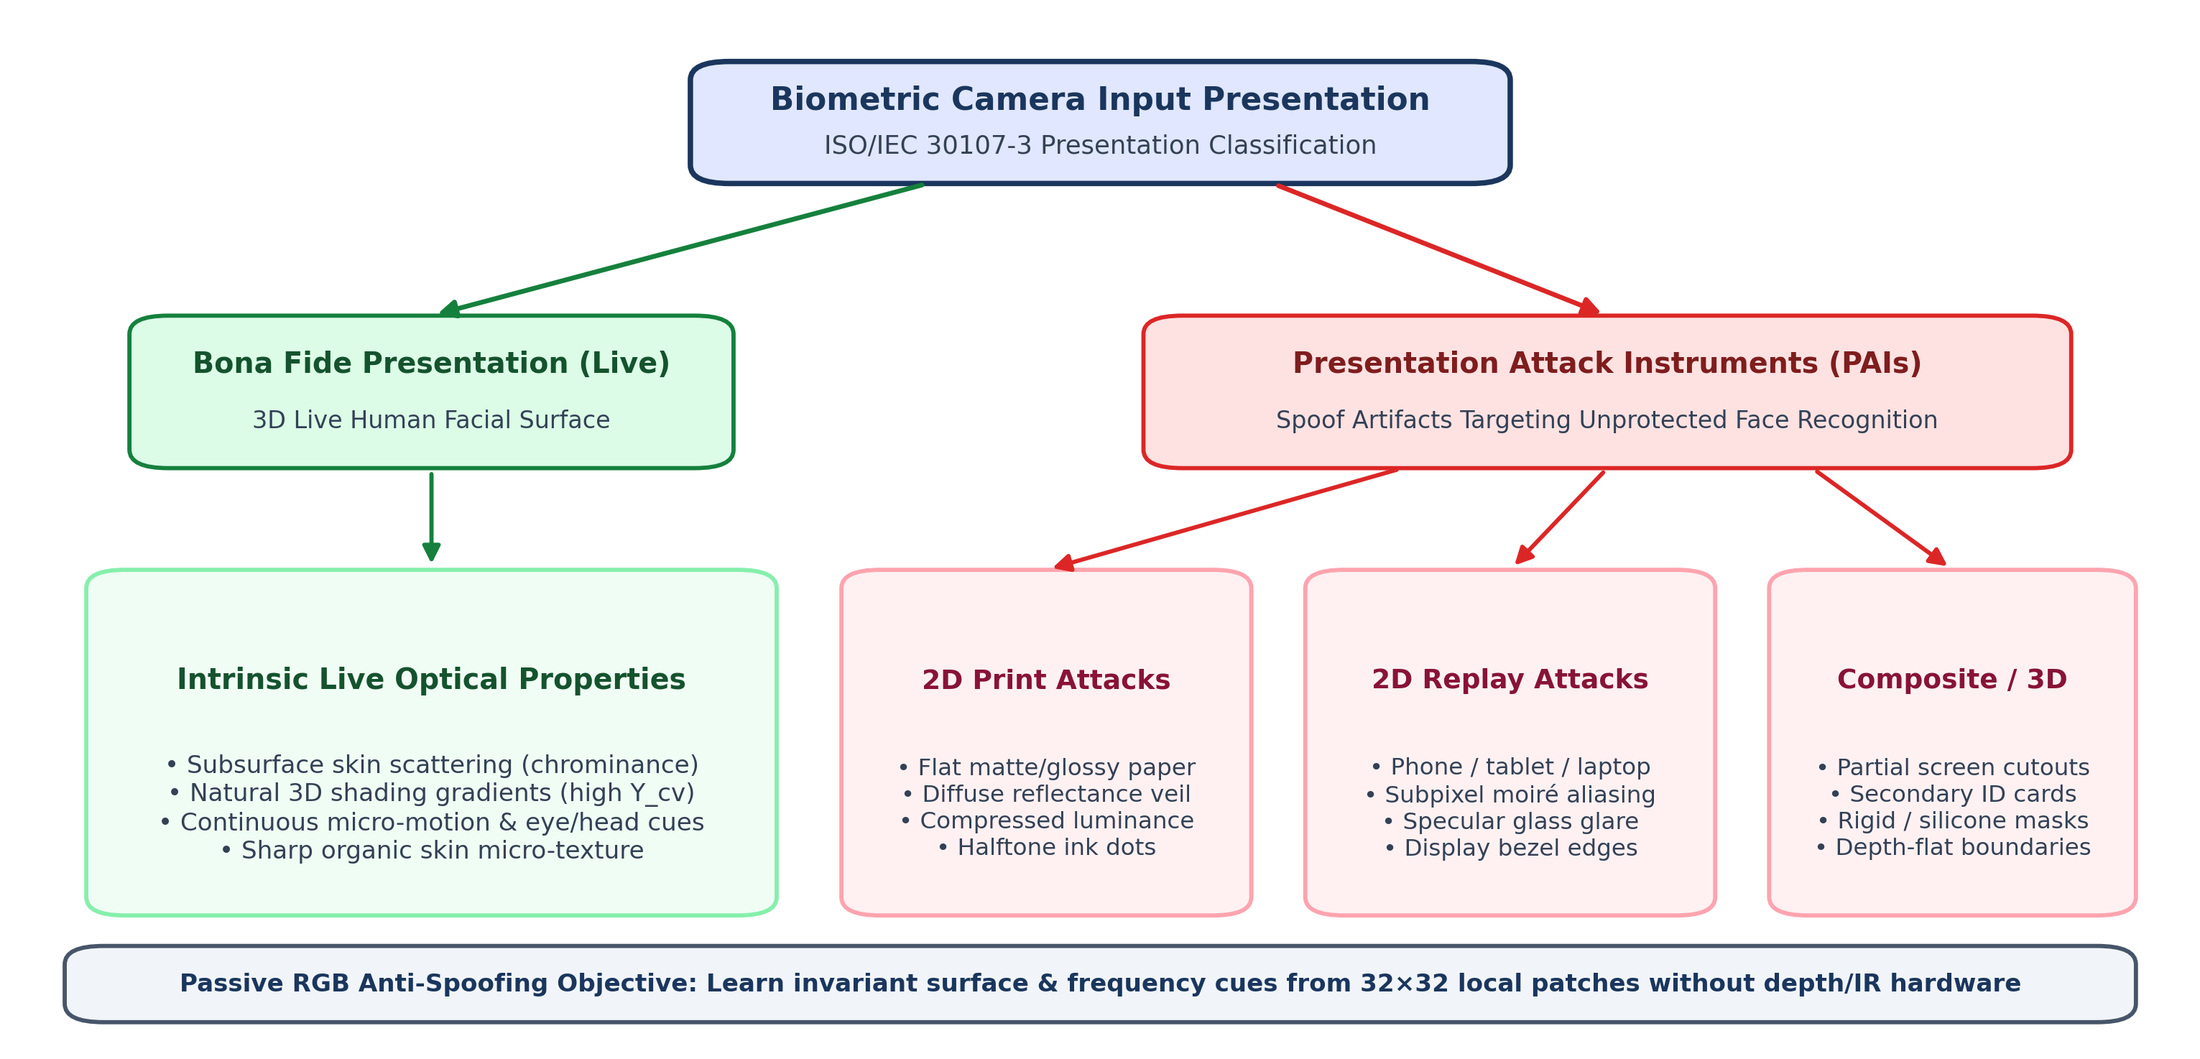
\includegraphics[width=0.96\textwidth]{Images/fig_pad_taxonomy.jpg}
\caption{ISO/IEC 30107-3 biometric presentation classification and passive RGB optical cues distinguishing bona fide faces from presentation attack instruments.}
\label{fig:pad_taxonomy}
\end{figure}

PAD systems are further categorized as \emph{active} or \emph{passive}. Active methods require explicit user participation---such as blinking on cue, turning the head toward a target angle, or reading randomized digits---which increases transaction time and remains vulnerable to edited video replays or deepfake puppetry~\cite{yu2023deep}. Passive PAD operates transparently on incoming video frames, extracting intrinsic physical and frequency-domain signatures within a fraction of a second.

\subsection{Optical and Chrominance Distortion Cues in Monocular RGB}

Although a commodity RGB sensor does not measure metric depth directly, recapturing a face from an intermediate display or paper substrate introduces measurable radiometric distortions~\cite{wen2015face, boulkenafet2016face}:
\begin{enumerate}
    \item \textbf{Subsurface scattering versus planar emission/reflection:} Live human skin is a multi-layered translucent medium in which incident light penetrates the epidermis and scatters through hemoglobin- and melanin-rich dermal layers before exiting. This produces smooth, continuous chrominance transitions in luminance-decoupled spaces such as $YC_rC_b$ and HSV. Conversely, printed paper exhibits a diffuse surface reflectance veil with compressed dynamic range (low luminance coefficient of variation), while electronic screens emit quantized RGB primaries restricted to the display panel's color gamut.
    \item \textbf{Spatial frequency aliasing and moir\'{e} interference:} Projecting discrete display subpixel grids (LCD RGB stripes or OLED PenTile matrices) onto a discrete CMOS camera sensor array generates high-frequency beat patterns (moir\'{e} fringes) and unnatural directional gradients when sampled at close range.
    \item \textbf{Specular glass reflections and planar shading:} Glass-covered mobile displays act as partial mirrors, superimposing sharp specular highlights of indoor ceiling fixtures onto facial regions, whereas three-dimensional facial geometry distributes shading continuously across the nasal bridge, zygomatic arches, and forehead.
\end{enumerate}

\subsection{Single-Stage Face Detection and Open-Set Verification}

A complete biometric attendance system combines three distinct visual tasks: (i) \emph{face detection}, which regresses bounding boxes and facial landmarks across spatial scales to isolate candidate regions of interest (ROIs); (ii) \emph{presentation attack detection}, which estimates the posterior probability that each localized ROI originates from a live face; and (iii) \emph{open-set face verification}, which maps an aligned facial crop onto a unit hypersphere so that identities can be enrolled from reference videos without retraining the recognition backbone~\cite{deng2019arcface}. Separating liveness estimation from identity recognition enables modular upgrades and ensures that spoof rejection remains invariant to whether an attacked identity is newly enrolled.

\section{Mathematical and Theoretical Basis}
\label{sec:mathematical_basis}

\subsection{Convolutional Feature Extraction and Receptive Fields}

Let $\mathbf{X} \in \mathbb{R}^{H \times W \times C_{\text{in}}}$ denote an input tensor of height $H$, width $W$, and channel depth $C_{\text{in}}$ scaled to $[0, 1]$. A two-dimensional discrete convolutional layer parameterized by $C_{\text{out}}$ learnable filter banks $\mathbf{K}^{(m)} \in \mathbb{R}^{k_h \times k_w \times C_{\text{in}}}$ and biases $b^{(m)} \in \mathbb{R}$ computes output feature map $m \in \{1, \dots, C_{\text{out}}\}$ at spatial coordinate $(u, v)$ according to Equation~\eqref{eq:conv2d}:
\begin{equation}
\label{eq:conv2d}
    Z_{u, v, m} = b^{(m)} + \sum_{c=1}^{C_{\text{in}}} \sum_{p=0}^{k_h - 1} \sum_{q=0}^{k_w - 1} X_{s \cdot u + p - P_h,\, s \cdot v + q - P_w,\, c} \, K^{(m)}_{p, q, c},
\end{equation}
where $s$ is the spatial stride and $(P_h, P_w)$ denote zero-padding widths. For kernel size $k$, padding $P$, and stride $s$, the resulting spatial dimension along height (and analogously width) is given by Equation~\eqref{eq:spatial_dim}:
\begin{equation}
\label{eq:spatial_dim}
    H_{\text{out}} = \left\lfloor \frac{H + 2P - k}{s} \right\rfloor + 1.
\end{equation}

Following the architectural principle established by Simonyan and Zisserman~\cite{simonyan2015very}, stacking two consecutive $3\times3$ convolutional layers with unit stride ($s=1$) yields an effective $5\times5$ receptive field while inserting an intermediate nonlinear activation and requiring only $2 \times (3^2 C^2) = 18 C^2$ weights instead of $5^2 C^2 = 25 C^2$. Pointwise nonlinearity is introduced via the Rectified Linear Unit (ReLU) in Equation~\eqref{eq:relu}:
\begin{equation}
\label{eq:relu}
    \phi(z) = \max(0, z),
\end{equation}
which preserves non-vanishing unit gradients in the positive half-space while inducing sparse activations. Overfitting on compact datasets is mitigated during training via inverted Dropout~\cite{srivastava2014dropout}, which multiplies hidden activations by independent Bernoulli masks $r_j \sim \text{Bernoulli}(1 - p_{\text{drop}})$ scaled by $(1 - p_{\text{drop}})^{-1}$.

At the classification head, raw logits $\mathbf{g} = [g_{\text{fake}}, g_{\text{real}}]^\top \in \mathbb{R}^2$ are mapped onto the probability simplex via the Softmax operator in Equation~\eqref{eq:softmax}:
\begin{equation}
\label{eq:softmax}
    P(y = c \mid \mathbf{X}) = \hat{y}_c = \frac{\exp(g_c)}{\sum_{k \in \{\text{fake}, \text{real}\}} \exp(g_k)}, \quad c \in \{\text{fake}, \text{real}\}.
\end{equation}
Given one-hot ground-truth targets $\mathbf{y}_i = [y_{i,0}, y_{i,1}]^\top \in \{0, 1\}^2$ across a mini-batch of $B$ crops and optional non-negative sample weights $w_i > 0$, parameters $\theta$ are optimized by minimizing the weighted categorical cross-entropy loss in Equation~\eqref{eq:cce}:
\begin{equation}
\label{eq:cce}
    \mathcal{L}_{\text{CCE}}(\theta) = -\frac{1}{B} \sum_{i=1}^{B} w_i \sum_{c=0}^{1} y_{i,c} \log \left(\hat{y}_{i,c}(\mathbf{X}_i; \theta)\right).
\end{equation}

\subsection{Feature Normalization Under Multi-Source Covariate Shift}

Internal activation distributions shift continuously during gradient-based training. Batch Normalization (BN)~\cite{ioffe2015batch} standardizes each channel $c$ across the mini-batch and spatial grid $\Omega = \{1, \dots, H\} \times \{1, \dots, W\}$ of cardinality $M = B \cdot H \cdot W$:
\begin{equation}
\label{eq:batchnorm}
    \mu_{\mathcal{B}, c} = \frac{1}{M} \sum_{i=1}^{B} \sum_{(u,v) \in \Omega} Z^{(i)}_{u,v,c}, \qquad
    \sigma^2_{\mathcal{B}, c} = \frac{1}{M} \sum_{i=1}^{B} \sum_{(u,v) \in \Omega} \left(Z^{(i)}_{u,v,c} - \mu_{\mathcal{B}, c}\right)^2,
\end{equation}
followed by an affine transformation $\tilde{Z}^{(i)}_{u,v,c} = \gamma_c (Z^{(i)}_{u,v,c} - \mu_{\mathcal{B}, c}) / \sqrt{\sigma^2_{\mathcal{B}, c} + \epsilon} + \beta_c$ with learnable scale $\gamma_c$ and shift $\beta_c$. Crucially, during training BN maintains exponential moving averages (EMA) for test-time inference according to Equation~\eqref{eq:bn_ema}:
\begin{equation}
\label{eq:bn_ema}
    \bar{\mu}_c^{(t)} = \alpha \, \bar{\mu}_c^{(t-1)} + (1 - \alpha)\, \mu_{\mathcal{B}, c}^{(t)}, \qquad
    \bar{\sigma}_c^{2\,(t)} = \alpha \, \bar{\sigma}_c^{2\,(t-1)} + (1 - \alpha)\, \sigma_{\mathcal{B}, c}^{2\,(t)},
\end{equation}
where $\alpha \in (0, 1)$ is the momentum coefficient (typically $0.99$).

Equations~\eqref{eq:cce}--\eqref{eq:bn_ema} expose a critical failure mechanism when merging imbalanced multi-camera datasets: scalar loss weights $w_i$ rescale parameter gradients $\nabla_\theta \mathcal{L}_{\text{CCE}}$ toward minority-domain samples, yet $\mu_{\mathcal{B}, c}$ and $\sigma^2_{\mathcal{B}, c}$ in Equation~\eqref{eq:batchnorm} remain \emph{unweighted} arithmetic averages dominated by the majority source. Consequently, convolutional weights co-adapt to batch-normalized activations whose statistics reflect the majority camera, producing severe threshold miscalibration at inference time.

Group Normalization (GN)~\cite{wu2018group} eliminates batch-composition dependence entirely by partitioning the $C$ channels of each individual sample $i$ into $G$ groups and normalizing strictly within sample-local index sets $\mathcal{S}_{i, g} = \{(u, v, k) : (u, v) \in \Omega,\, \lfloor k / (C/G) \rfloor = g\}$:
\begin{equation}
\label{eq:groupnorm}
    \mu_{\text{GN}}(i, g) = \frac{1}{|\mathcal{S}_{i,g}|} \sum_{(u,v,k) \in \mathcal{S}_{i,g}} Z^{(i)}_{u,v,k}, \qquad
    \sigma^2_{\text{GN}}(i, g) = \frac{1}{|\mathcal{S}_{i,g}|} \sum_{(u,v,k) \in \mathcal{S}_{i,g}} \left(Z^{(i)}_{u,v,k} - \mu_{\text{GN}}(i, g)\right)^2.
\end{equation}
For one-dimensional dense layers where spatial dimensions collapse ($H=W=1$), setting $G=1$ recovers Layer Normalization (LN)~\cite{ba2016layer}, computing statistics identically during training and single-sample inference without moving averages.

\subsection{Adaptive Optimization and Weight-Space Interpolation}

Network parameters are updated via the Adam optimizer~\cite{kingma2015adam}, which tracks bias-corrected first and second gradient moments $(\hat{\mathbf{m}}_t, \hat{\mathbf{v}}_t)$ with decay rates $(\beta_1, \beta_2)$ and step size $\eta$ as shown in Equation~\eqref{eq:adam}:
\begin{equation}
\label{eq:adam}
    \mathbf{m}_t = \beta_1 \mathbf{m}_{t-1} + (1 - \beta_1)\mathbf{g}_t, \quad
    \mathbf{v}_t = \beta_2 \mathbf{v}_{t-1} + (1 - \beta_2)\mathbf{g}_t^{\odot 2}, \quad
    \theta_t = \theta_{t-1} - \eta \frac{\mathbf{m}_t / (1 - \beta_1^t)}{\sqrt{\mathbf{v}_t / (1 - \beta_2^t)} + \epsilon}.
\end{equation}

When adapting a broadly trained anchor model $\theta_{\text{anchor}}$ to a specialized target-camera distribution yielding fine-tuned weights $\theta_{\text{ft}}$, unconstrained fine-tuning can erode out-of-distribution robustness on secondary cameras. Weight-Space Ensembling for Fine-Tuning (WiSE-FT)~\cite{wortsman2022robust} linearly interpolates parameters within shared basin geometry according to Equation~\eqref{eq:wiseft}:
\begin{equation}
\label{eq:wiseft}
    \theta^*(\lambda) = (1 - \lambda)\,\theta_{\text{anchor}} + \lambda\,\theta_{\text{ft}}, \quad \lambda \in [0, 1],
\end{equation}
achieving target-domain accuracy gains while retaining multi-camera invariance at zero additional inference cost.

\subsection{Optical Quality, Spatial Tracking, Verification, and PAD Metrics}

\noindent\textbf{Defocus Estimation:} Motion and out-of-focus blur attenuate high-frequency screen moir\'{e} and skin pore cues, causing blurred bona fide faces to resemble low-resolution replays. Sharpness on a grayscale crop $I_g$ is quantified by the variance of the discrete Laplacian operator~\cite{pech2000diatom} in Equation~\eqref{eq:laplacian}:
\begin{equation}
\label{eq:laplacian}
\begin{aligned}
    \nabla^2 I_g(u, v) &= I_g(u+1,v) + I_g(u-1,v) + I_g(u,v+1) + I_g(u,v-1) - 4I_g(u,v), \\
    \sigma^2_{\text{Lap}} &= \text{Var}_{u,v}\!\left(\nabla^2 I_g(u,v)\right).
\end{aligned}
\end{equation}

\noindent\textbf{Bounding-Box Association:} Across consecutive video frames, detected face boxes $B_a = (x_1^a, y_1^a, x_2^a, y_2^a)$ and active tracks $B_b = (x_1^b, y_1^b, x_2^b, y_2^b)$ are matched via Intersection-over-Union ($\text{IoU}$) in Equation~\eqref{eq:iou}:
\begin{equation}
\label{eq:iou}
    \text{IoU}(B_a, B_b) = \frac{\max(0, \min(x_2^a, x_2^b) - \max(x_1^a, x_1^b)) \cdot \max(0, \min(y_2^a, y_2^b) - \max(y_1^a, y_1^b))}{\text{Area}(B_a) + \text{Area}(B_b) - \text{Area}(B_a \cap B_b)}.
\end{equation}

\noindent\textbf{Angular-Margin Verification:} For identity recognition, ArcFace~\cite{deng2019arcface} normalizes both embedding vectors $\hat{\mathbf{e}}_i = \mathbf{e}_i / \|\mathbf{e}_i\|_2 \in \mathbb{R}^{512}$ and class weight centers $\hat{\mathbf{W}}_j = \mathbf{W}_j / \|\mathbf{W}_j\|_2$, enforcing an additive angular margin penalty $m$ with feature scale $s$ during backbone pretraining (Equation~\eqref{eq:arcface}):
\begin{equation}
\label{eq:arcface}
    \mathcal{L}_{\text{Arc}} = -\frac{1}{N} \sum_{i=1}^{N} \log \frac{\exp\!\left(s \cos(\theta_{y_i} + m)\right)}{\exp\!\left(s \cos(\theta_{y_i} + m)\right) + \sum_{j \neq y_i} \exp\!\left(s \cos \theta_j\right)}, \quad \theta_j = \arccos\!\left(\hat{\mathbf{W}}_j^\top \hat{\mathbf{e}}_i\right).
\end{equation}
At attendance inference time, matching a query embedding $\hat{\mathbf{q}}$ against a gallery of $\ell_2$-normalized prototype vectors $\{\hat{\mathbf{p}}_k\}_{k=1}^{K}$ reduces to maximum inner-product cosine similarity in Equation~\eqref{eq:cosine_sim}:
\begin{equation}
\label{eq:cosine_sim}
    s_{\max}(\hat{\mathbf{q}}) = \max_{1 \le k \le K} \left(\hat{\mathbf{q}}^\top \hat{\mathbf{p}}_k\right),
\end{equation}
accepting the identity associated with the winning prototype if and only if $s_{\max}(\hat{\mathbf{q}}) \ge \tau$ and the upstream anti-spoofing gate classifies the presentation as bona fide.

\noindent\textbf{ISO/IEC 30107-3 PAD Error Rates:} Letting $\text{TP}_{\text{real}}$ and $\text{FN}_{\text{real}}$ denote bona fide presentations classified as real and fake, and letting $\text{TN}_{\text{fake}}$ and $\text{FP}_{\text{fake}}$ denote spoof attacks classified as fake and real, standardized PAD performance is governed by Attack Presentation Classification Error Rate ($\text{APCER}$), Bona Fide Presentation Classification Error Rate ($\text{BPCER}$), and Average Classification Error Rate ($\text{ACER}$) in Equation~\eqref{eq:iso_metrics}:
\begin{equation}
\label{eq:iso_metrics}
    \text{APCER} = \frac{\text{FP}_{\text{fake}}}{\text{TN}_{\text{fake}} + \text{FP}_{\text{fake}}}, \quad
    \text{BPCER} = \frac{\text{FN}_{\text{real}}}{\text{TP}_{\text{real}} + \text{FN}_{\text{real}}}, \quad
    \text{ACER} = \frac{\text{APCER} + \text{BPCER}}{2}.
\end{equation}

\section{Existing Frameworks and Algorithms}
\label{sec:exist_frameworks_algorithms}

Deploying an integrated real-time anti-spoofing and attendance pipeline requires selecting compatible face detectors, PAD classifiers, recognition backbones, and CPU execution runtimes. Table~\ref{tab:algorithms} compares the principal algorithmic candidates across these four layers.

\begin{table}[htbp]
\centering
\caption{Technical comparison of candidate detection, anti-spoofing, verification, and inference frameworks.}
\label{tab:algorithms}
\footnotesize
\begin{tabular}{L{2.8cm}L{2.3cm}L{4.3cm}L{4.5cm}}
\toprule
\textbf{Algorithm / Engine} & \textbf{Subsystem} & \textbf{Technical Advantages} & \textbf{Constraints / Trade-offs} \\
\midrule
ResNet-10 SSD~\cite{liu2016ssd} & Face Detection & Consistent tight facial crop geometry on $300\times300$ inputs; mature OpenCV Caffe DNN support. & Lacks native 5-point landmarks; higher false positives on background clutter than anchor-free detectors. \\
\addlinespace[1.5pt]
YuNet ONNX~\cite{wu2023yunet} & Face Detection & Tiny footprint ($<250$~KB); millisecond CPU latency; outputs 5 facial landmarks for eye-span quality checks. & Slightly looser default bounding-box margins than Caffe SSD unless aligned. \\
\addlinespace[1.5pt]
SCRFD~\cite{guo2022scrfd} & Face Detection & Computation redistribution yields high recall across scales; paired natively with InsightFace alignment. & Bounding-box aspect ratio differs from SSD/YuNet crops, requiring ROI re-alignment before PAD scoring. \\
\addlinespace[1.5pt]
Colour-LBP~\cite{boulkenafet2016face} & Face PAD & Handcrafted $YC_bC_r$/HSV histograms; zero GPU requirement; transparent feature space. & Degrades sharply on high-density OLED panels and uncalibrated webcam AWB shifts. \\
\addlinespace[1.5pt]
CDCN~\cite{yu2020searching} / Aux-Depth~\cite{liu2018learning} & Face PAD & Captures fine-grained central gradient differences and pseudo-3D facial curvature. & Dense $32\times32$ depth supervision and multi-level fusion incur substantial CPU latency per frame. \\
\addlinespace[1.5pt]
PatchNet~\cite{wang2022patchnet} & Face PAD & Enforces local surface patch discrimination; resists global subject identity memorization. & Requires center-crop/scale-jitter pretext formulation and ResNet-18-scale backbone compute. \\
\addlinespace[1.5pt]
\texttt{LivenessNet} (VGG-style~\cite{simonyan2015very}) & Face PAD & $545{,}154$ parameters ($2.15$~MiB); $32\times32$ patch input inherently suppresses identity detail; $0.163$~ms CPU inference. & Small receptive scale lacks global context (e.g., hand holding phone bezel) unless paired with temporal/ROI logic. \\
\addlinespace[1.5pt]
ArcFace (ResNet-50)~\cite{deng2019arcface} & Verification & Geodesic angular margin yields highly separable $512$-D unit embeddings for few-shot video enrollment. & Completely vulnerable to 2D print and screen replay without an external PAD gate. \\
\addlinespace[1.5pt]
LiteRT + XNNPACK~\cite{david2021tensorflow} & CPU Runtime & Fuses Conv+BN layers into static flatbuffers; vectorizes $3\times3$ kernels on x86 AVX2/FMA CPUs. & Requires static graph freezing; dynamic Python training callbacks are unavailable post-export. \\
\bottomrule
\end{tabular}
\end{table}

\subsection{Face Detection Frameworks}

Single Shot MultiBox Detector (SSD)~\cite{liu2016ssd} with a reduced ResNet-10 backbone processes $300\times300$ mean-subtracted BGR blobs and produces stable, tightly cropped facial boxes well suited for offline training crop generation. For live streaming and quality gating, YuNet~\cite{wu2023yunet} employs depthwise separable convolutions and an anchor-free head to regress both bounding boxes and five facial keypoints (left/right eye centers, nose tip, mouth corners) in a few milliseconds on CPU. Within the attendance recognition stack, Sample and Computation Redistribution for Face Detection (SCRFD)~\cite{guo2022scrfd} reallocates FLOPs toward shallow feature pyramid stages, supplying accurate 5-point landmarks for similarity-transform alignment into $112\times112$ ArcFace inputs.

\subsection{Passive Anti-Spoofing Architectures and Runtime Compilers}

While deep auxiliary networks such as CDCN~\cite{yu2020searching} and multi-channel CNNs~\cite{george2020biometric} excel on GPU benchmarks, CPU-bound attendance kiosks benefit from compact VGG-style~\cite{simonyan2015very} or MobileNetV3-style~\cite{howard2019searching} designs operating on low-resolution facial patches. Consistent with the patch-level hypothesis of PatchNet~\cite{wang2022patchnet}, downsampling a localized face box to $32\times32$~pixels discards fine biometric identity structures (such as iris patterns or mole placement) while retaining macro-radiometric and screen-aliasing cues across color channels. Furthermore, compiling a Keras convolutional graph into a frozen LiteRT (\texttt{.tflite}) model~\cite{david2021tensorflow} folds Batch Normalization scale and offset parameters directly into preceding convolution weights, eliminating Python dispatch overhead and enabling sub-millisecond SIMD execution via XNNPACK.

\section{Limitations and Research Motivation}
\label{sec:limitations_motivation}

Synthesizing the theoretical analysis in Section~\ref{sec:mathematical_basis} and the framework survey in Section~\ref{sec:exist_frameworks_algorithms} reveals four concrete failure modes that frequently undermine lightweight passive anti-spoofing systems in practice:
\begin{enumerate}
    \item \textbf{Optimistic evaluation via frame-level leakage:} Adjacent frames extracted from a $30$~FPS video share nearly identical background illumination, subject identity, and sensor noise. Random frame-level train/test splits allow compact CNNs to memorize session-specific color casts, reporting $>99\%$ laboratory accuracy while failing on unseen subjects ($\text{ACER} > 25\%$).
    \item \textbf{Normalization drift in multi-source training:} Combining a large legacy webcam archive with smaller target-camera recordings using inverse-frequency sample weights introduces severe mismatch between unweighted Batch Normalization moving statistics (Equation~\eqref{eq:bn_ema}) and weighted gradient updates (Equation~\eqref{eq:cce}).
    \item \textbf{Detector geometry and compression confounding:} Mixing videos across file containers (\texttt{.mov} vs.\ \texttt{.mp4}) or swapping face detectors between training (SSD) and deployment (SCRFD) introduces spurious domain shortcuts and crop-scale shifts that degrade live recognition gating.
    \item \textbf{Single-frame decision volatility:} Evaluating Equation~\eqref{eq:softmax} independently on every video frame exposes interactive check-in terminals to momentary specular glare and motion blur, causing rapid label oscillation or transient false accepts.
\end{enumerate}

Addressing the first three challenges requires a disciplined data acquisition, optical filtering, and person-disjoint partitioning pipeline before any model optimization takes place. Chapter~\ref{chap:data_processing} details how raw video streams were collected, cleaned, audited, and structured to establish a leakage-free foundation.

\chapter{Data Processing}
\label{chap:data_processing}

Reliable passive face anti-spoofing depends as heavily on dataset hygiene and split isolation as on neural network design. When training data contain unmasked background faces, severe defocus blur, container-format shortcuts, or subject overlap across splits, compact convolutional models rapidly latch onto spurious correlations that collapse during live deployment. This chapter documents the multi-phase self-collected video cohorts, region-of-interest (ROI) extraction rules, optical quality filters, patch representation choices, and person-disjoint validation protocols constructed for this study.

\section{Dataset Description}
\label{sec:dataset_description}

\subsection{General Information}
\label{subsec:dataset_general}

All anti-spoofing and attendance datasets employed in this project are self-collected indoor video corpora acquired under realistic office and classroom illumination. Rather than relying on a single static archive, data collection evolved across three structured cohorts designed to expose and eliminate specific generalization bottlenecks:

\begin{enumerate}
    \item \textbf{Cohort I --- Legacy Webcam Archive (\texttt{dataset/}):} The initial corpus comprises $33$ indoor webcam recordings ($720$p/$1080$p) of bona fide users and handheld screen replay attacks, yielding $24{,}221$ extracted facial crops ($13{,}773$ \texttt{fake} and $10{,}448$ \texttt{real}). Auditing this archive revealed that prior random frame-level splits placed nearly identical consecutive frames into both training and test sets. Re-partitioning the $33$ videos cleanly at the video level established a leakage-free baseline, but subsequent testing on external subjects revealed sharp cross-subject degradation due to limited demographic and presentation diversity.
    \item \textbf{Cohort II --- Multi-Subject Expansion and Merged Multi-Source Benchmark:} To broaden subject diversity, $56$ additional videos ($30$ \texttt{real}, $26$ \texttt{fake}; $1.58$~GB total) were recorded across distinct volunteer identities under varied indoor lighting and mobile display angles. Combining $4{,}925$ unrestricted crops from these $56$ videos with $24{,}032$ quality-verified crops from Cohort~I produced an $89$-video \textbf{Merged Multi-Source Benchmark} ($28{,}957$ crops across two distinct acquisition sources). While invaluable for diagnosing multi-source Batch Normalization drift, diagnostic audits uncovered subtle acquisition confounders between cohorts---most notably QuickTime (\texttt{.mov}) versus MPEG-4 (\texttt{.mp4}) compression characteristics and detector crop-margin differences.
    \item \textbf{Cohort III --- Target-Sensor \texttt{Cam4K} Benchmark (\texttt{dataset\_cam4k/}):} To eliminate cross-container and cross-detector confounding entirely, a dedicated benchmark of $91$ high-definition/4K videos ($44$ \texttt{real}, $47$ \texttt{fake}) was recorded directly on the target deployment sensor: a commercial \textbf{USB SC-M200 camera}. Every recording was stored uniformly in \texttt{.mp4} format and partitioned physically by human subject prior to frame extraction. Scanning $140{,}707$ raw video frames produced $26{,}094$ clean $32\times32$ BGR facial crops ($12{,}618$ \texttt{real}, $13{,}476$ \texttt{fake}). To verify cross-camera retention, an auxiliary external set of $600$ crops ($300$ \texttt{real}, $300$ \texttt{fake}) was captured on an integrated laptop webcam. In parallel, multi-clip bona fide enrollment videos ($2$--$3$ clips per employee) were recorded to calibrate the \texttt{ChamCong\_FaceID} recognition gallery.
\end{enumerate}

\subsection{Statistical Overview}
\label{subsec:dataset_stats}

Table~\ref{tab:dataset_cohorts} summarizes the scale, sensor characteristics, and experimental role of every dataset cohort utilized across the project lifecycle.

\begin{table}[htbp]
\centering
\caption{Overview of video cohorts and evaluation sets used across experimental phases.}
\label{tab:dataset_cohorts}
\small
\begin{tabular}{L{3.5cm}L{2.5cm}R{1.4cm}R{1.8cm}L{4.5cm}}
\toprule
\textbf{Dataset Cohort} & \textbf{Sensor / Format} & \textbf{Videos} & \textbf{Face Crops} & \textbf{Primary Experimental Role} \\
\midrule
Cohort I: Legacy Baseline & USB/Laptop (\texttt{.mp4/\allowbreak.mov}) & $33$ & $24{,}221$ & Expose frame-split leakage; establish clean video-disjoint baseline. \\
\addlinespace[3pt]
Cohort IIa: Quality-Gated Expansion & Multi-device (\texttt{.mov/\allowbreak.mp4}) & $56$ & $7{,}029$ & Multi-subject generalization test \& $12$~s continuous session replay. \\
\addlinespace[3pt]
Cohort IIb: Merged Multi-Source & Dual-source heterogeneous & $89$ & $28{,}957$ & Controlled ablation of BatchNorm drift vs.\ stratified GroupNorm. \\
\addlinespace[3pt]
Cohort III: \texttt{Cam4K} Benchmark & USB SC-M200 (\texttt{.mp4}) & $91$ & $26{,}094$ & Primary person-disjoint training, validation, and unseen test benchmark. \\
\addlinespace[3pt]
External Cross-Cam Set & Integrated Laptop Cam & --- & $600$ & Out-of-domain sensor retention verification ($300$ real, $300$ fake). \\
\bottomrule
\end{tabular}
\end{table}

Because Cohort~III (\texttt{Cam4K}) serves as the definitive production benchmark on target hardware, Table~\ref{tab:cam4k_splits} provides its exact split-level composition extracted from \texttt{extraction\_manifest.json}. Across all three person-disjoint partitions, class priors remain closely balanced ($47.35\%$ \texttt{real} vs.\ $52.65\%$ \texttt{fake} in training; $49.23\%$ \texttt{real} vs.\ $50.77\%$ \texttt{fake} in validation; and $50.84\%$ \texttt{real} vs.\ $49.16\%$ \texttt{fake} in testing), preventing majority-class decision bias.

\begin{table}[htbp]
\centering
\caption{Detailed person-disjoint split statistics of the target-sensor \texttt{Cam4K} dataset ($140{,}707$ raw frames scanned with temporal stride $5$).}
\label{tab:cam4k_splits}
\small
\begin{tabular}{L{2.3cm}R{1.5cm}R{1.5cm}R{1.5cm}R{1.85cm}R{1.85cm}R{1.85cm}}
\toprule
\textbf{Partition} & \textbf{Real Videos} & \textbf{Fake Videos} & \textbf{Total Videos} & \textbf{Real Crops} & \textbf{Fake Crops} & \textbf{Total Crops} \\
\midrule
Training (\texttt{train}) & $30$ & $33$ & $63$ & $7{,}703$ & $8{,}565$ & $16{,}268$ \\
Validation (\texttt{val}) & $7$ & $7$ & $14$ & $2{,}469$ & $2{,}546$ & $5{,}015$ \\
Testing (\texttt{test}) & $7$ & $7$ & $14$ & $2{,}446$ & $2{,}365$ & $4{,}811$ \\
\midrule
\textbf{Total} & $\mathbf{44}$ & $\mathbf{47}$ & $\mathbf{91}$ & $\mathbf{12{,}618}$ & $\mathbf{13{,}476}$ & $\mathbf{26{,}094}$ \\
\bottomrule
\end{tabular}
\end{table}

\subsection{Data Visualization}
\label{subsec:dataset_vis}

Figure~\ref{fig:dataset_samples} displays ten representative $32\times32$ facial crops drawn from the Legacy Webcam and SC-M200 (\texttt{Cam4K}) cohorts, upsampled solely for print legibility. Visual inspection highlights both intra-class diversity (age groups, eyewear, head yaw, and indoor backgrounds) and characteristic presentation attack artifacts: electronic replay crops exhibit elevated high-key screen luminance, subtle chromatic shifts toward blue-magenta display backlights, and reduced micro-shadow contrast along the nasolabial folds compared to bona fide skin.

\begin{figure}[htbp]
\centering
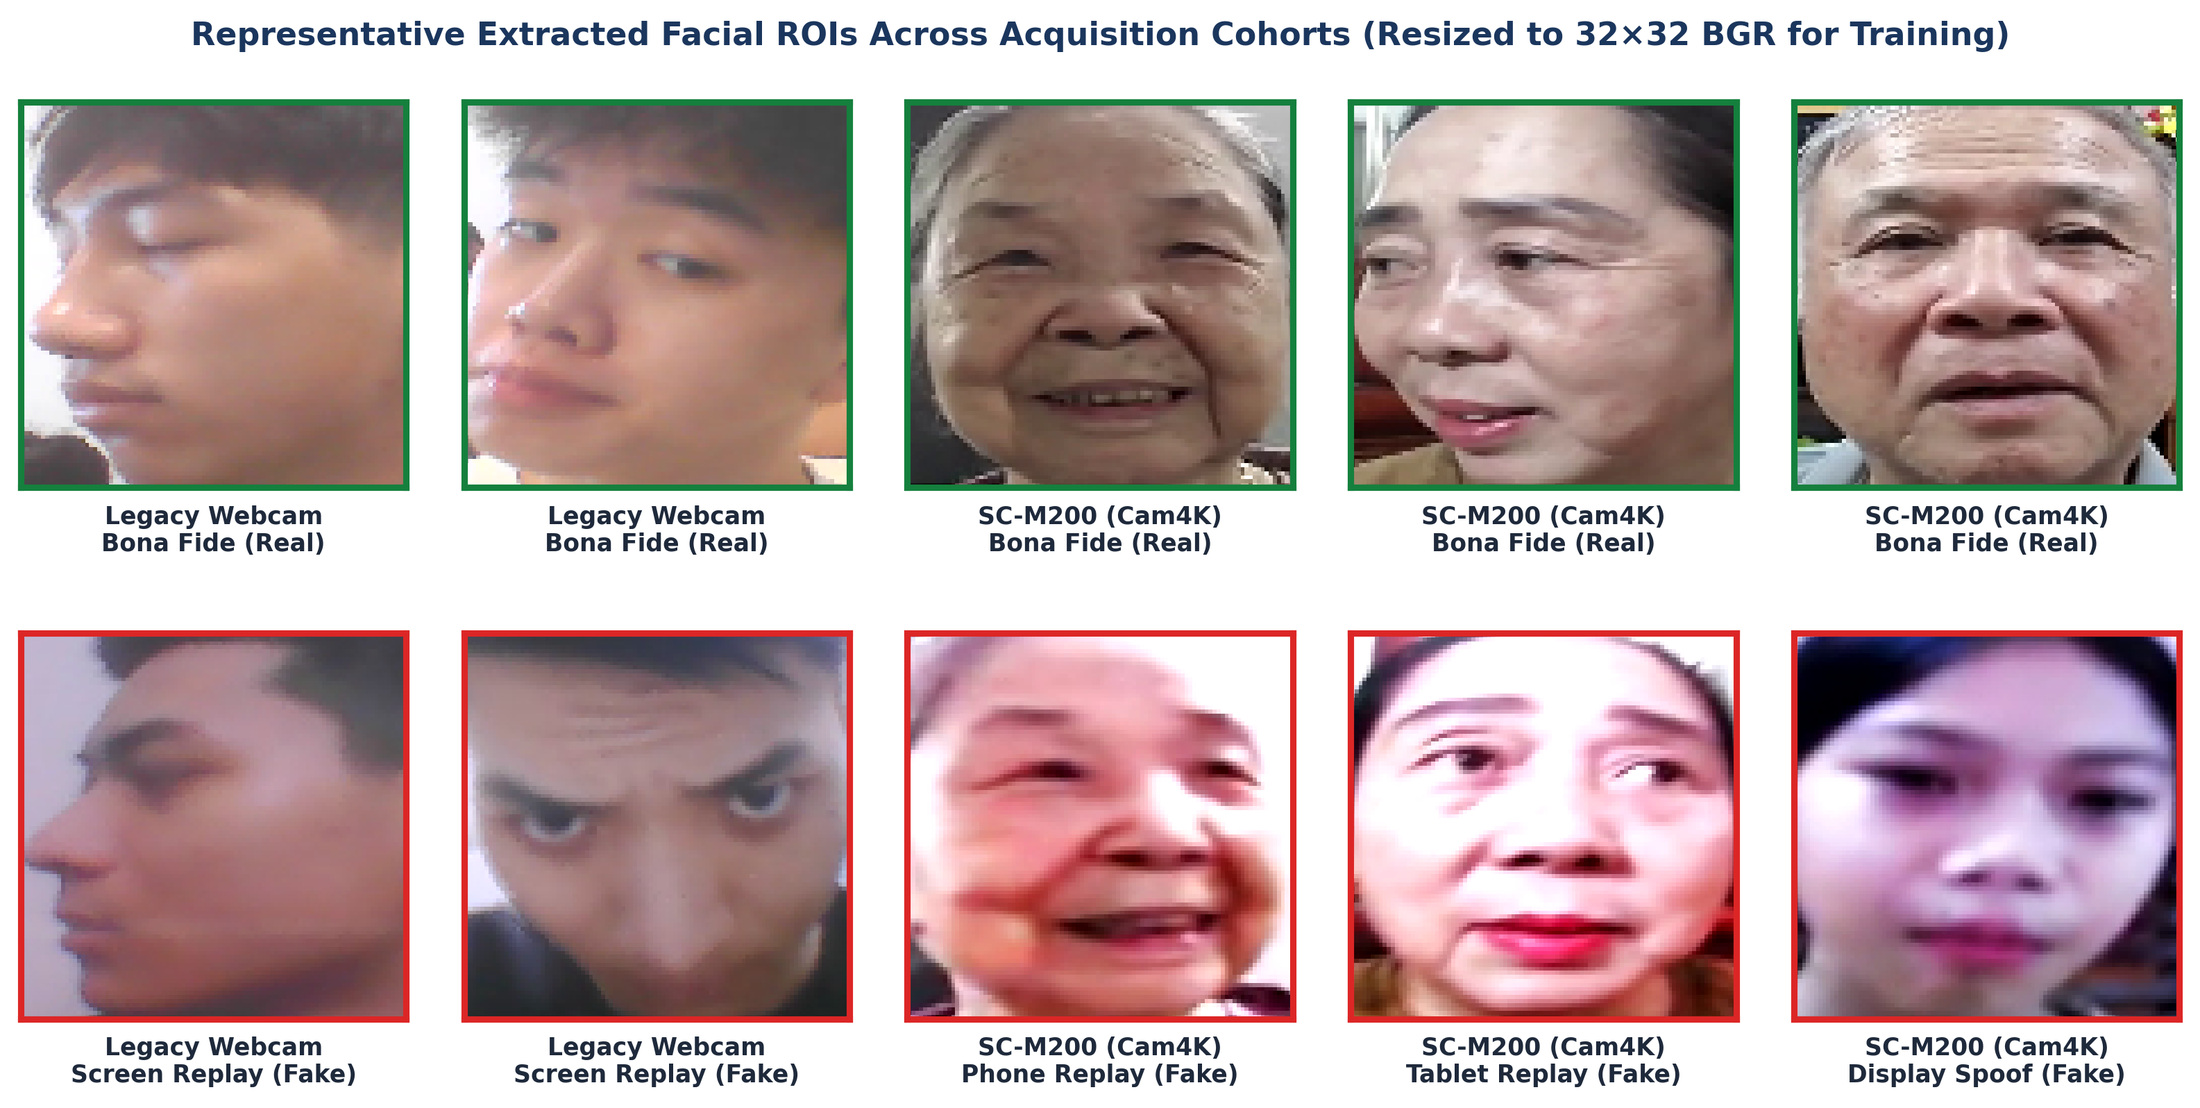
\includegraphics[width=0.96\textwidth]{Images/fig_dataset_samples.jpg}
\caption{Representative extracted facial ROIs across acquisition cohorts resized to $32\times32$ BGR inputs. Top row (green border): bona fide live subjects. Bottom row (red border): smartphone, tablet, and monitor replay attacks.}
\label{fig:dataset_samples}
\end{figure}

Figure~\ref{fig:dataset_statistics} illustrates the structural balance of the \texttt{Cam4K} corpus. Figure~\ref{fig:dataset_statistics}(a) confirms near-parity between bona fide and spoof crops across all three subject-disjoint splits. Figure~\ref{fig:dataset_statistics}(b) plots the per-video crop count distribution across all $91$ videos under temporal stride $5$: both real and fake recordings average $286.7$ extracted crops per video (spanning approximately $55$ to $435$ crops depending on clip duration), motivating video-balanced epoch sampling during training so longer clips do not dominate gradient updates.

\begin{figure}[htbp]
\centering
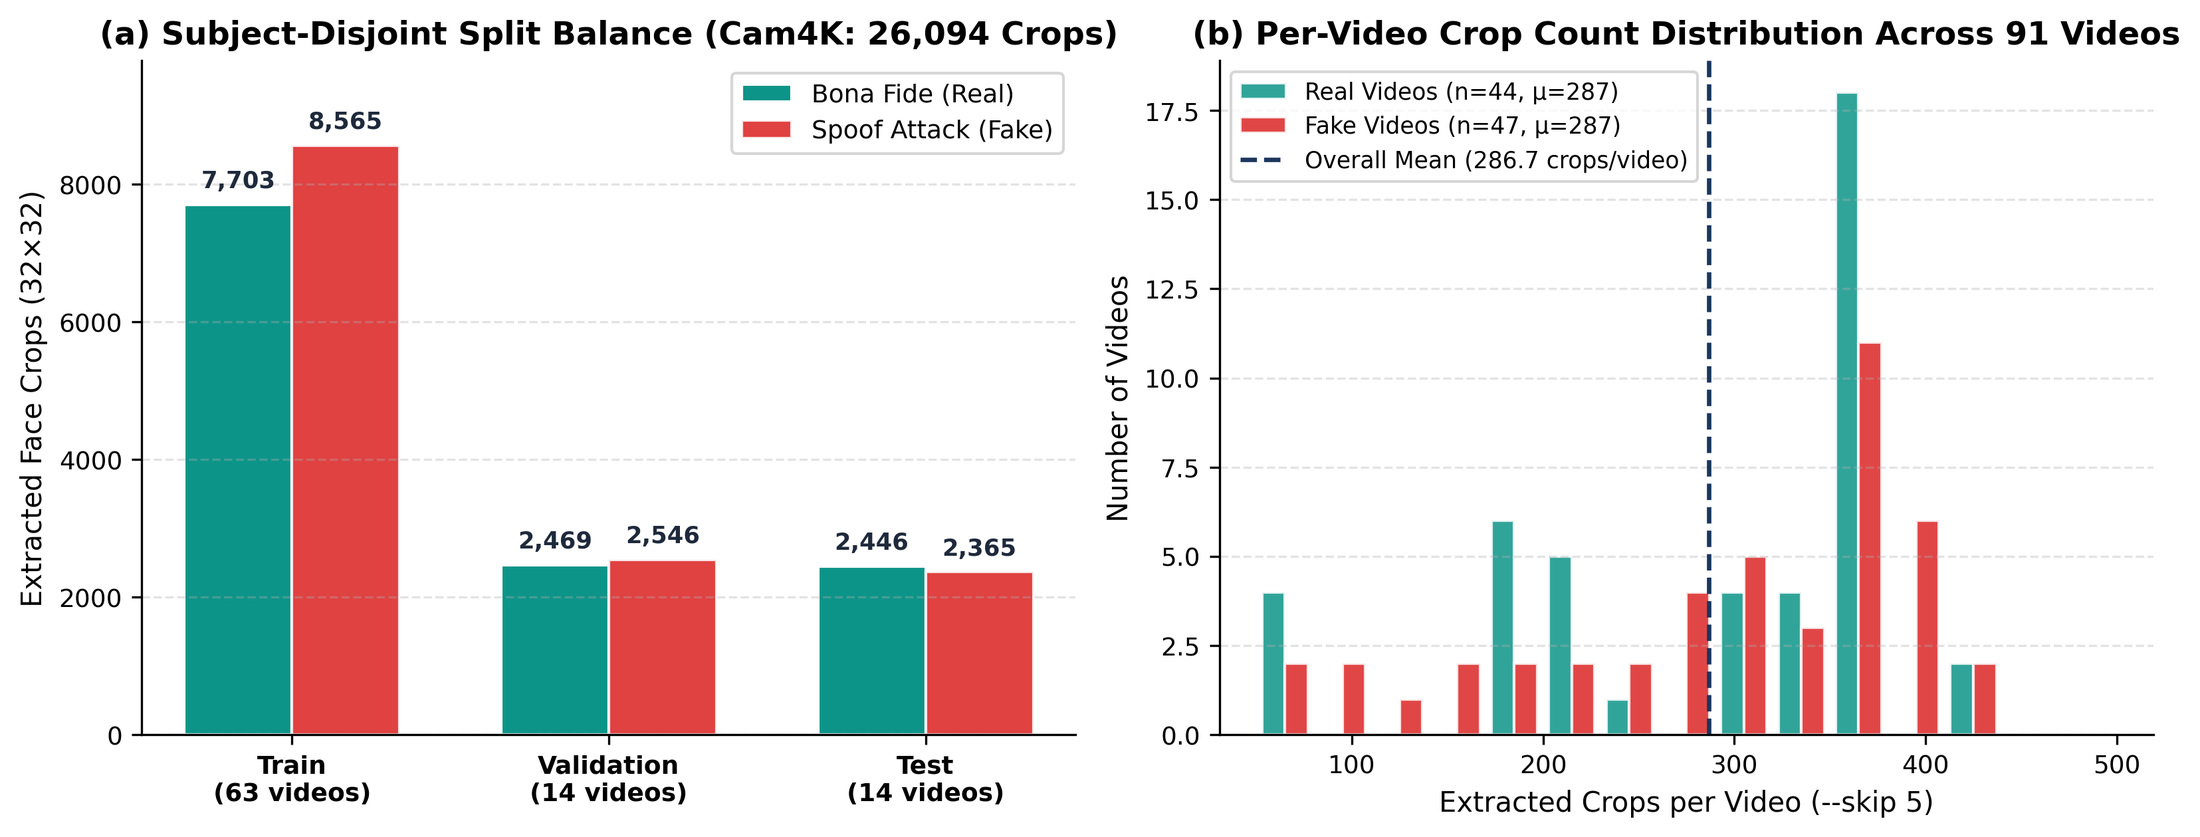
\includegraphics[width=0.98\textwidth]{Images/fig_dataset_statistics.jpg}
\caption{Statistical distribution of the \texttt{Cam4K} benchmark: (a) bona fide versus spoof crop counts across person-disjoint splits; (b) histogram of extracted crops per video across $91$ SC-M200 recordings.}
\label{fig:dataset_statistics}
\end{figure}

\section{Data Preprocessing and Cleaning}
\label{sec:data_preprocessing}

Transforming raw multi-megabyte video streams into clean, supervision-consistent neural network inputs follows a deterministic five-step preprocessing pipeline implemented across \texttt{scripts/extract\_cam4k.py}, \texttt{face\_extract.py}, and \texttt{ChamCong\_FaceID/preprocessing.py}.

\subsection{Temporal Subsampling and Detector Alignment}

Consecutive frames in a $30$~FPS video stream differ minimally in facial pose and illumination. During offline extraction on \texttt{Cam4K}, only every fifth frame (\texttt{--skip 5}, corresponding to $6$~Hz temporal sampling) is evaluated, reducing raw frame volume from $140{,}707$ decoded frames to $26{,}094$ saved crops in $452.6$~seconds while preserving full pose trajectories across each clip. Each sampled frame is resized to $300\times300$, mean-subtracted by $(104.0, 177.0, 123.0)$, and passed through the Caffe ResNet-10 SSD face detector~\cite{liu2016ssd} with confidence threshold $0.50$. When multiple candidate boxes exceed threshold, only the highest-confidence foreground detection with side dimensions $\ge 20$~px is retained.

\subsection{Spatial Masking of Contaminating Presenter Faces}

Manual audit of wide-angle 4K spoof recordings uncovered a subtle label-corruption hazard: in three early attack videos (\texttt{fake\_REC-0001-A.mp4}, \texttt{fake\_REC-0002-A.mp4}, and \texttt{fake\_REC-0003-A.mp4}), the person holding the presentation smartphone stood partially inside the right periphery of the camera field of view. Whenever the smartphone screen tilted momentarily and suffered specular glare, the face detector assigned higher confidence to the live presenter's face on the right edge than to the spoof screen, injecting genuine live faces into the \texttt{fake} training directory. To eliminate this contamination deterministically, \texttt{extract\_cam4k.py} applies a spatial right-edge zero-mask ($I[:, \lfloor 0.65 W \rfloor : W] \leftarrow 0$) prior to face detection on affected wide-angle recordings, guaranteeing that $100\%$ of extracted \texttt{fake} ROIs originate strictly from the attack instrument.

\subsection{Six-Stage Optical Quality Filtering}

During multi-source dataset curation and employee gallery enrollment, raw detections pass through a six-rule optical quality gate grounded in the sharpness formulation of Equation~\eqref{eq:laplacian}~\cite{pech2000diatom}:
\begin{enumerate}
    \item \textbf{Minimum spatial resolution:} Bounding-box width and height must satisfy $\min(w, h) \ge 65$~px for anti-spoofing crops ($\ge 80$~px for ArcFace enrollment) so downsampling does not amplify sensor shot noise.
    \item \textbf{Boundary completeness:} Boxes clipped against frame borders ($x_1 < 0$, $y_1 < 0$, $x_2 > W$, or $y_2 > H$) are discarded to prevent partial-face distortion.
    \item \textbf{Landmark geometry:} When YuNet 5-point keypoints are available, all five landmarks must lie strictly inside the bounding box and the Euclidean inter-ocular distance must satisfy $d_{\text{eye}} \ge 0.12\,w$, filtering extreme profile poses and false background detections.
    \item \textbf{Underexposure floor:} Mean grayscale intensity across the ROI must satisfy $\mu_{\text{gray}} \ge 35$ (on $[0, 255]$) to reject severely shadowed frames where chrominance ratios degenerate into quantization noise.
    \item \textbf{Specular glare ceiling:} The fraction of saturated pixels ($I_{\text{gray}} > 245$) must not exceed $0.45$, preventing washed-out overhead ceiling reflections from masking facial texture.
    \item \textbf{Defocus and motion-blur rejection:} The ROI is standardized to $128\times128$ grayscale so pixel-grid spacing is scale-invariant, and crops with discrete Laplacian variance $\sigma^2_{\text{Lap}} < 12.0$ ($< 45.0$ for high-precision gallery enrollment) are rejected. Applying this audit retroactively to Cohort~I identified and removed $189$ corrupted legacy crops ($158$ excessive glare and $31$ severe motion blur).
\end{enumerate}

\subsection{Normalization, Encoding, and Photometric Augmentation}

Accepted BGR facial crops are bilinearly resized to $32\times32\times3$ and linearly normalized to floating-point $[0, 1]$ by dividing pixel intensities by $255.0$. Class labels are encoded alphabetically via \texttt{LabelEncoder} (\texttt{fake} $\mapsto 0 \mapsto [1, 0]^\top$, \texttt{real} $\mapsto 1 \mapsto [0, 1]^\top$) and persisted alongside model weights as \texttt{le\_cam4k.pickle}.

To prevent overfitting to static camera mounting geometry or fixed indoor color temperatures, training mini-batches undergo online stochastic augmentation strictly on the training split (validation and test splits remain completely unaugmented):
\begin{itemize}
    \item \textbf{Geometric perturbation:} Random in-plane rotation within $\pm 10^\circ$, horizontal and vertical translation up to $8\%$ of patch dimensions, isotropic zoom within $[0.92, 1.08]$, nearest-border fill, and $50\%$ horizontal mirroring.
    \item \textbf{Per-channel white-balance jitter:} Applied with probability $0.35$, each BGR channel $c \in \{B, G, R\}$ is independently transformed as $\tilde{X}_{u,v,c} = \text{clip}(\alpha_c X_{u,v,c} + \delta_c,\, 0,\, 1)$ with gain $\alpha_c \sim \mathcal{U}(0.92, 1.08)$ and offset $\delta_c \sim \mathcal{U}(-0.03, 0.03)$, simulating sensor-to-sensor Automatic White Balance variations.
\end{itemize}

\section{Feature Representation and Patch Scale Rationale}
\label{sec:feature_extraction}

A deliberate design choice in this pipeline is representing each detected face as a $32\times32\times3$ BGR tensor ($3{,}072$ scalar values) for anti-spoofing while retaining $112\times112\times3$ landmark-aligned crops for ArcFace identity verification. This dual-scale representation serves two complementary purposes:
\begin{enumerate}
    \item \textbf{Implicit identity suppression for PAD:} High-resolution facial inputs ($224\times224$) encourage small datasets ($60$--$90$ subjects) to memorize person-specific biometric traits (eyebrow shape, scars, eyeglasses). Downsampling to $32\times32$ acts as a structural low-pass bottleneck on fine identity geometry while preserving regional color-channel ratios, screen backlight halos, and macro-aliasing gradients learned by \texttt{LivenessNet}'s $3\times3$ convolutional filters~\cite{wang2022patchnet}.
    \item \textbf{Complementary optical chrominance cues:} For deployments enabling multi-cue print protection (\texttt{fusion=True}), the pipeline additionally computes explicit statistical descriptors in $YC_rC_b$ and HSV spaces over the central facial skin patch ($[0.18h : 0.85h,\, 0.18w : 0.82w]$): red-chrominance dispersion $\sigma(C_r)$, mean saturation $\mu(S)$, luminance coefficient of variation $\sigma(Y)/(\mu(Y)+1)$, and bright-veil excess $P_{92}(Y) - P_{50}(Y)$, targeting matte paper prints whose desaturated diffuse reflectance differs from self-illuminated screens.
    \item \textbf{Metric-space prototype representation for attendance:} In \texttt{ChamCong\_FaceID}, verified enrollment frames are aligned via 5-point similarity transformation to $112\times112$ and projected through the pretrained InsightFace ResNet-50 backbone~\cite{deng2019arcface} into $\ell_2$-normalized $512$-dimensional vectors. Rather than collapsing all frames of an employee into a single global centroid that blurs lighting differences, enrollment computes both per-video normalized prototypes and a person-level centroid, storing them in \texttt{face\_db.npz}.
\end{enumerate}

\section{Data Validation and Splitting Strategy}
\label{sec:splitting_strategy}

To guarantee unbiased generalization estimates, strict hierarchical data isolation rules were enforced and verified programmatically prior to training:
\begin{itemize}
    \item \textbf{Person-disjoint physical partitioning:} In Cohort~III (\texttt{Cam4K}), raw video files were assigned to \texttt{train/} ($63$ videos, $69.2\%$), \texttt{validate/} ($14$ videos, $15.4\%$), and \texttt{test/} ($14$ videos, $15.4\%$) directories by human identity before running \texttt{extract\_cam4k.py}. No subject appearing in the $14$ test videos appears in either training or validation sets.
    \item \textbf{Programmatic leakage and duplicate audits:} Every training run serializes a split manifest (\texttt{split.json}) recording video stems and frame counts per partition, executing set-intersection assertions ($\mathcal{V}_{\text{train}} \cap \mathcal{V}_{\text{val}} = \emptyset$, $\mathcal{V}_{\text{train}} \cap \mathcal{V}_{\text{test}} = \emptyset$, $\mathcal{V}_{\text{val}} \cap \mathcal{V}_{\text{test}} = \emptyset$). In the $89$-video Merged Multi-Source Benchmark, SHA-256 cryptographic hashes of raw pixel buffers were also cross-checked across splits to verify zero duplicate frames.
    \item \textbf{Deterministic reproducibility:} Partitioning, queue shuffling, and bootstrap confidence-interval resampling use fixed pseudo-random seeds (\texttt{seed = 42}) across Python, NumPy, and TensorFlow so every split and metric reported in Chapter~\ref{chap:results} is bit-for-bit auditable.
\end{itemize}

\section{Summary of Data Processing}
\label{sec:data_summary}

In summary, the data processing pipeline progressed from an audited $33$-video legacy archive and an $89$-video multi-source diagnostic corpus to a clean, target-sensor $91$-video \texttt{Cam4K} benchmark containing $26{,}094$ person-disjoint $32\times32$ BGR facial crops. Automated temporal stride sampling, spatial right-edge holder masking, six-stage optical quality gating, and white-balance-aware augmentation ensure that training supervision reflects genuine physical presentation cues rather than background artifacts or sensor shortcuts. Chapter~\ref{chap:methodology} builds directly upon these curated datasets to specify the \texttt{LivenessNet} neural architecture, balanced training and weight-interpolation algorithms, real-time LiteRT CPU engine, and attendance verification system.

\chapter{Methodology}
\label{chap:methodology}

This chapter presents the architectural design, training algorithms, inference optimizations, and system integration strategies developed to achieve passive real-time face anti-spoofing on commodity CPU hardware. Building upon the theoretical formulations in Chapter~\ref{chap:theoretical_background} and the curated person-disjoint datasets in Chapter~\ref{chap:data_processing}, every component from neural layer topology to multi-threaded camera scheduling and WebSocket attendance gating is specified in reproducible detail.

\section{Overall Workflow}
\label{sec:overall_workflow}

Figure~\ref{fig:workflow} depicts the end-to-end engineering workflow, organized into an offline model preparation pipeline (Stage~1) and a unified online runtime serving three operational channels (Stage~2).

\begin{figure}[htbp]
\centering
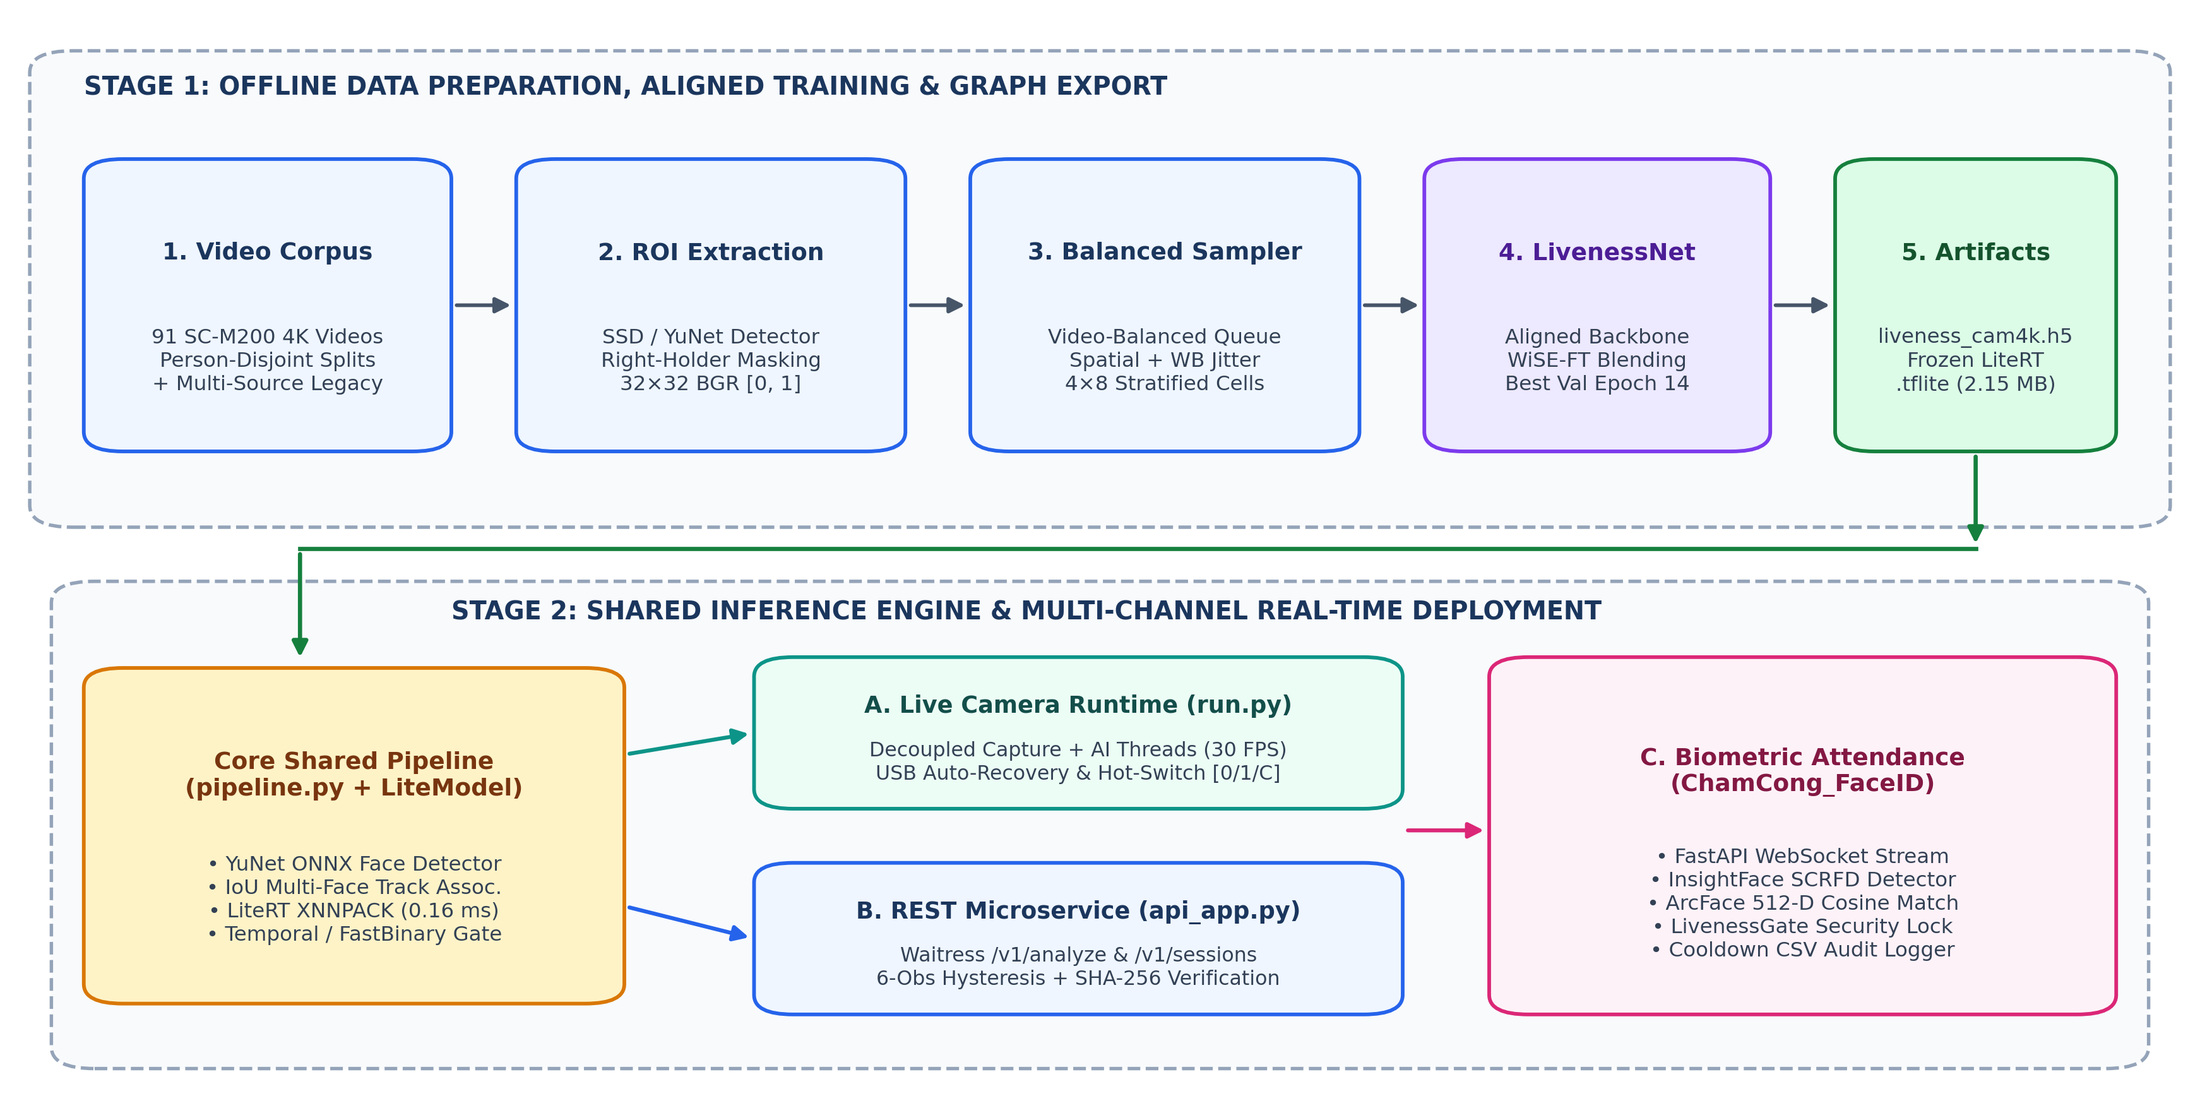
\includegraphics[width=0.98\textwidth]{Images/fig_system_workflow.jpg}
\caption{End-to-end system workflow comprising Stage~1 (offline ROI extraction, balanced training, WiSE-FT head interpolation, and LiteRT export) and Stage~2 (shared CPU inference pipeline powering live camera UI, REST microservice, and biometric attendance verification).}
\label{fig:workflow}
\end{figure}

In \textbf{Stage~1}, person-disjoint raw videos from the SC-M200 \texttt{Cam4K} benchmark and multi-source legacy archives undergo automated ROI localization, presenter-face spatial masking, and six-stage quality filtering to produce normalized $32\times32\times3$ BGR patches. A video-balanced mini-batch generator feeds \texttt{LivenessNet} under geometric and per-channel white-balance jitter. Rather than retraining early spatial filters from scratch on a single sensor, the convolutional feature extractor is anchored to universal multi-source weights while the dense classification head is adapted to the SC-M200 distribution and blended via WiSE-FT~\cite{wortsman2022robust}. The selected Epoch~$14$ checkpoint is serialized both as a standard Keras artifact (\texttt{liveness\_cam4k.h5}) and as a frozen LiteRT flatbuffer (\texttt{liveness\_cam4k.tflite}).

In \textbf{Stage~2}, a single shared inference engine (\texttt{pipeline.py} coupled with \texttt{LiteModel}) executes YuNet ONNX face detection, greedy $\text{IoU}$ multi-face track association, $0.163$~ms XNNPACK CNN scoring, and temporal smoothing. This shared core eliminates training-serving skew across three deployment targets: (A) an interactive $30$~FPS desktop camera monitor (\texttt{run.py}), (B) a stateless/stateful HTTP microservice (\texttt{api\_app.py}), and (C) the \texttt{ChamCong\_FaceID} WebSocket biometric attendance application.

\section{System Design and Architecture}
\label{sec:system_architecture}

\subsection{\texttt{LivenessNet} Convolutional Architecture and Normalization Variants}

To satisfy sub-millisecond CPU latency constraints while preventing subject-identity memorization on $32\times32$ patches, \texttt{LivenessNet} (\texttt{model/livenessnet.py}) adopts a compact VGG-inspired~\cite{simonyan2015very} sequential topology with progressively expanding channel widths ($32 \to 64 \to 128$) and aggressive spatial downsampling ($32 \to 10 \to 5 \to 2$). Figure~\ref{fig:model_architecture} illustrates the block-level tensor flow, and Table~\ref{tab:livenessnet_layers} enumerates every layer, output dimension, and parameter count.

\begin{figure}[htbp]
\centering
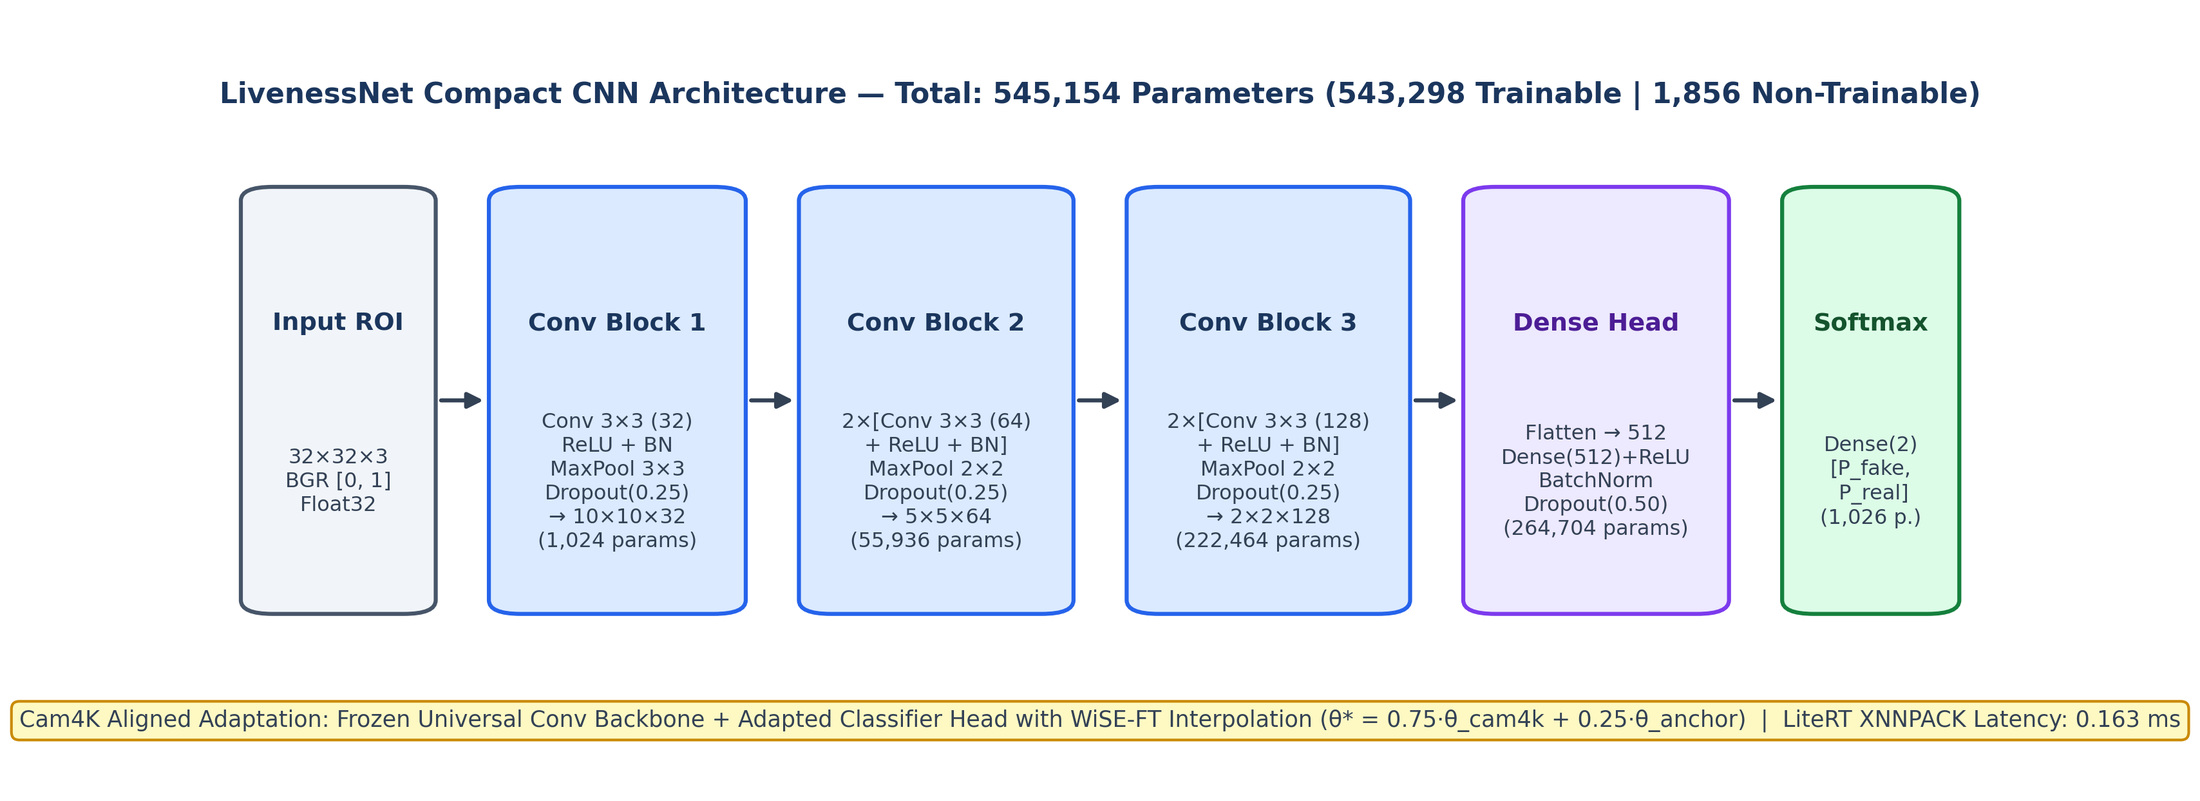
\includegraphics[width=0.98\textwidth]{Images/fig_livenessnet_arch.jpg}
\caption{Block diagram of the $545{,}154$-parameter \texttt{LivenessNet} CNN architecture, highlighting spatial downsampling across three convolutional blocks, the $512$-unit classifier head, and WiSE-FT aligned transfer.}
\label{fig:model_architecture}
\end{figure}

\begin{table}[htbp]
\centering
\caption{Layer-by-layer specification of \texttt{LivenessNet} (input tensor $32 \times 32 \times 3$, channels-last).}
\label{tab:livenessnet_layers}
\small
\begin{tabular}{L{2.3cm}L{3.9cm}L{2.8cm}L{2.3cm}R{2.1cm}}
\toprule
\textbf{Stage} & \textbf{Layer / Operation} & \textbf{Kernel / Config} & \textbf{Output Shape} & \textbf{Parameters} \\
\midrule
Input & Normalized BGR Patch & $\text{float32} \in [0, 1]$ & $32 \times 32 \times 3$ & $0$ \\
\midrule
\multirow{3}{*}{Conv Block 1} & \texttt{Conv2D} + \texttt{ReLU} & $32 \times (3\times3)$, \texttt{same} & $32 \times 32 \times 32$ & $896$ \\
 & \texttt{BatchNormalization} & $\text{axis}=-1$ & $32 \times 32 \times 32$ & $128$ \\
 & \texttt{MaxPooling2D} + \texttt{Dropout} & Pool $3\times3$, $p=0.25$ & $10 \times 10 \times 32$ & $0$ \\
\midrule
\multirow{5}{*}{Conv Block 2} & \texttt{Conv2D} + \texttt{ReLU} & $64 \times (3\times3)$, \texttt{same} & $10 \times 10 \times 64$ & $18{,}496$ \\
 & \texttt{BatchNormalization} & $\text{axis}=-1$ & $10 \times 10 \times 64$ & $256$ \\
 & \texttt{Conv2D} + \texttt{ReLU} & $64 \times (3\times3)$, \texttt{same} & $10 \times 10 \times 64$ & $36{,}928$ \\
 & \texttt{BatchNormalization} & $\text{axis}=-1$ & $10 \times 10 \times 64$ & $256$ \\
 & \texttt{MaxPooling2D} + \texttt{Dropout} & Pool $2\times2$, $p=0.25$ & $5 \times 5 \times 64$ & $0$ \\
\midrule
\multirow{5}{*}{Conv Block 3} & \texttt{Conv2D} + \texttt{ReLU} & $128 \times (3\times3)$, \texttt{same} & $5 \times 5 \times 128$ & $73{,}856$ \\
 & \texttt{BatchNormalization} & $\text{axis}=-1$ & $5 \times 5 \times 128$ & $512$ \\
 & \texttt{Conv2D} + \texttt{ReLU} & $128 \times (3\times3)$, \texttt{same} & $5 \times 5 \times 128$ & $147{,}584$ \\
 & \texttt{BatchNormalization} & $\text{axis}=-1$ & $5 \times 5 \times 128$ & $512$ \\
 & \texttt{MaxPooling2D} + \texttt{Dropout} & Pool $2\times2$, $p=0.25$ & $2 \times 2 \times 128$ & $0$ \\
\midrule
\multirow{4}{*}{Classifier Head} & \texttt{Flatten} & --- & $512$ & $0$ \\
 & \texttt{Dense} + \texttt{ReLU} & $512$ units & $512$ & $262{,}656$ \\
 & \texttt{BatchNorm} + \texttt{Dropout} & $\text{axis}=-1$, $p=0.50$ & $512$ & $2{,}048$ \\
 & \texttt{Dense} + \texttt{Softmax} & $2$ units ($[P_{\text{fake}}, P_{\text{real}}]$) & $2$ & $1{,}026$ \\
\midrule
\multicolumn{4}{l}{\textbf{Total Parameters} ($543{,}298$ trainable + $1{,}856$ non-trainable BN stats)} & $\mathbf{545{,}154}$ \\
\bottomrule
\end{tabular}
\end{table}

Block~1 applies a single $3\times3$ convolution followed by $3\times3$ max pooling (Equation~\eqref{eq:spatial_dim}: $\lfloor (32 - 3)/3 \rfloor + 1 = 10$), immediately compressing spatial redundancy while capturing local chromatic edges and specular highlights. Blocks~2 and~3 each stack two $3\times3$ convolutions before $2\times2$ pooling, expanding the effective receptive field across almost the entire $32\times32$ patch to detect screen-border gradients and moir\'{e} periodicity. Flattening the $2\times2\times128$ tensor yields a $512$-dimensional descriptor, ensuring direct dimensional matching into the $512$-unit fully connected layer ($262{,}656$ weights, accounting for $48.2\%$ of total model capacity).

To support heterogeneous multi-source training without Batch Normalization moving-average drift (analyzed mathematically in Equations~\eqref{eq:batchnorm}--\eqref{eq:groupnorm}), \texttt{LivenessNet.build()} implements a configurable normalization switch (\texttt{norm\_type}):
\begin{itemize}
    \item \texttt{norm\_type="batch"}: Instantiates channel-wise \texttt{BatchNormalization} across all five convolutional layers and the $512$-unit dense layer; optimal when mini-batches are strictly balanced or when folding affine BN parameters into static LiteRT convolutions.
    \item \texttt{norm\_type="group"}: Replaces every convolutional normalizer with \texttt{GroupNormalization}~\cite{wu2018group} ($G = 8$ groups, i.e., $4$, $8$, and $16$ channels per group in Blocks~1--3) and replaces the dense normalizer with \texttt{LayerNormalization}~\cite{ba2016layer}, guaranteeing identical sample-local normalization between multi-domain training and single-frame inference ($543{,}298$ trainable parameters, $0$ non-trainable moving averages).
\end{itemize}

\subsection{Frozen LiteRT Compilation and XNNPACK Acceleration}

Calling \texttt{model.predict()} directly inside Keras~3 incurs substantial per-frame Python graph-dispatch overhead ($\approx 25$--$45$~ms per call on CPU), which bottlenecks real-time multi-face streaming. In \texttt{scripts/export\_web\_model.py} and \texttt{inference\_runtime.py} (\texttt{LiteModel}), the trained Keras network is traced via a concrete \texttt{tf.function} input signature ($\text{shape}=[1, 32, 32, 3]$, \texttt{tf.float32}) and compiled into a flatbuffer (\texttt{web\_models/liveness\_cam4k.tflite}, $2.18$~MB).

Crucially, post-training dynamic-range or \texttt{int8} quantization is deliberately omitted: empirical inspection confirmed that subtle high-frequency screen-replay artifacts produce small floating-point activation differences that quantization noise can blur, whereas the unquantized \texttt{float32} flatbuffer is already only $2.18$~MB and executes in $0.163$~ms on CPU via TensorFlow Lite's XNNPACK AVX2/FMA delegate~\cite{david2021tensorflow}.

\subsection{Decoupled Multi-Threaded Live Camera Runtime}

Standard synchronous OpenCV loops (\texttt{cap.read()} $\to$ inference $\to$ \texttt{cv2.imshow()}) stall camera buffer draining whenever neural detection runs, introducing visible display lag and USB frame drops. \texttt{LiveCameraRuntime} in \texttt{run.py} decouples acquisition, inference, and UI rendering across three concurrent execution paths:
\begin{enumerate}
    \item \textbf{Capture thread (\texttt{\_capture\_loop}):} Opens hardware cameras with MJPG four-character compression at $1280\times720$ and $30$~FPS (\texttt{CAP\_DSHOW} on Windows with automatic fallback to default backends), setting internal driver buffer depth to~$1$ and continuously overwriting a lock-protected latest-frame slot so stale frames are discarded immediately.
    \item \textbf{Hardware fault tolerance and virtual-camera guard:} Virtual smartphone webcam drivers (e.g., idle DroidCam feeds) emit solid orange/blue/black placeholder screens; \texttt{run.py} rejects candidate devices whose pixel standard deviation satisfies $\sigma_{\text{frame}} < 2.0$. Furthermore, loose high-bandwidth USB cables on 4K cameras occasionally drop packets; rather than terminating on a single failed read, the capture loop tolerates up to $50$ consecutive transient read misses ($10$~ms backoff) before triggering full automatic USB re-initialization, and supports instant keyboard hot-switching (\texttt{[0]}, \texttt{[1]}, \texttt{[C]}).
    \item \textbf{AI worker thread (\texttt{\_ai\_loop}):} Independently pulls the most recent frame Sequence ID, downscales the longest image edge to $\le 480$~px for fast YuNet localization, extracts $32\times32$ crops from the full-resolution frame, scores all faces in a single vectorized batch, and publishes bounding-box overlays to the $30$~FPS UI thread.
\end{enumerate}

\subsection{Production REST API Microservice Architecture}

For language-agnostic integration with external enterprise portals, \texttt{api\_app.py} exposes the shared pipeline over HTTP via the production Waitress WSGI server. Table~\ref{tab:api_endpoints} summarizes the versioned \texttt{/v1} endpoint contract.

\begin{table}[htbp]
\centering
\caption{REST API endpoint specification implemented in \texttt{api\_app.py}.}
\label{tab:api_endpoints}
\small
\begin{tabular}{L{1.6cm}L{4.8cm}L{7.7cm}}
\toprule
\textbf{Method} & \textbf{Endpoint Path} & \textbf{Operational Semantics and Security Controls} \\
\midrule
\texttt{GET} & \texttt{/v1/health} & Liveness probe returning \texttt{status: ok} and SHA-256 model digest. \\
\texttt{GET} & \texttt{/openapi.json} & Machine-readable OpenAPI~3.0.3 contract for client code generation. \\
\texttt{POST} & \texttt{/v1/analyze} & Stateless single-JPEG check; returns raw softmax scores and \texttt{decision\_ready: false} (requires multi-frame session for final verdict). \\
\texttt{POST} & \texttt{/v1/sessions} & Allocates isolated server-side \texttt{TemporalDecision} state ($30$~s TTL, LRU cap $64$). \\
\texttt{POST} & \texttt{/v1/sessions/\{id\}/frames} & Appends binary \texttt{image/jpeg} frame to session tracker; returns 7-state fail-closed verdict and per-face track diagnostics. \\
\texttt{DELETE} & \texttt{/v1/sessions/\{id\}} & Deterministically purges session track memory upon check-in completion. \\
\bottomrule
\end{tabular}
\end{table}

Two critical engineering safeguards harden the HTTP layer: first, payloads are restricted to raw binary \texttt{image/jpeg} ($\le 2$~MB, spatial bounds $32$--$1920$~px) decoded with \texttt{cv2.IMREAD\_IGNORE\_ORIENTATION} so EXIF rotation tags on mobile uploads cannot invert facial orientation relative to upright training crops; second, inference is guarded by a non-blocking mutex (\texttt{infer\_lock.acquire(blocking=False)}) that immediately returns HTTP~\texttt{429 Too Many Requests} (\texttt{Retry-After: 1}) under burst contention rather than queuing stale biometric frames.

\subsection{Biometric Attendance Architecture and Detector ROI Re-Alignment}

The capstone application \texttt{ChamCong\_FaceID} (\texttt{ChamCong\_FaceID/app.py}) integrates passive anti-spoofing directly into a real-time employee attendance terminal built with FastAPI and HTML5 WebSockets (\texttt{/ws}). Browser clients stream JPEG frames at $10$~FPS ($640\times480$) to the backend, which runs InsightFace \texttt{buffalo\_l} (SCRFD face detector~\cite{guo2022scrfd} + $512$-D ArcFace ResNet-50~\cite{deng2019arcface} on ONNX Runtime).

During integration testing, a crucial geometric domain shift was identified and solved inside \texttt{LivenessGate} (\texttt{ChamCong\_FaceID/liveness/liveness\_gate.py}): SCRFD regresses tighter vertical forehead/chin bounding boxes than the Caffe SSD and YuNet detectors used when curating \texttt{LivenessNet} training crops. Feeding raw SCRFD crops directly into \texttt{LivenessNet} shifted spatial scale at the $32\times32$ patch boundary. To restore exact geometric alignment, \texttt{LivenessGate} expands each SCRFD bounding box $(x_1, y_1, x_2, y_2)$ outward by a $15\%$ margin on all four sides, runs lightweight YuNet localization strictly within that padded sub-window to recover the canonical training-style face box (falling back to the SCRFD box only if YuNet returns empty), scores the aligned $32\times32$ crop with \texttt{liveness\_cam4k.tflite}, and smooths probabilities through \texttt{FastBinaryDecision}.

Attendance authorization follows a strict fail-closed conjunctive rule:
\begin{enumerate}
    \item If \texttt{LivenessGate} classifies the track as \texttt{fake}, verification is aborted immediately, rendering a red bounding box labeled \texttt{[FAKE] <Matched Name>} with banner \texttt{FAKE - TU CHOI} and writing zero records to the attendance log.
    \item Only when the track is verified as \texttt{real} AND the maximum cosine similarity (Equation~\eqref{eq:cosine_sim}) against enrolled employee prototypes satisfies $s_{\max}(\hat{\mathbf{q}}) \ge \tau = 0.55$ does the system check a per-employee $30$-second anti-duplicate cooldown timer and append a timestamped record (\texttt{Name}, \texttt{Date}, \texttt{Time}, \texttt{Confidence}) to \texttt{attendance\_YYYY-MM-DD.csv}.
\end{enumerate}

\section{Algorithm Description}
\label{sec:algorithm_description}

\subsection{Video-Balanced Aligned Training and WiSE-FT Interpolation}

Standard epoch iteration over extracted image folders weights each training video proportionally to its frame count, allowing longer recordings to dominate gradient updates. Algorithm~\ref{alg:training} formalizes the aligned training procedure implemented in \texttt{scripts/train\_cam4k.py}.

\begin{algorithm}[htbp]
\caption{Video-Balanced Aligned Transfer Training with WiSE-FT Head Interpolation}
\label{alg:training}
\small
\begin{algorithmic}[1]
\Require Person-disjoint video crop pools $\{\mathcal{D}_{c, v}\}$ for class $c \in \{\text{fake}, \text{real}\}$ and video $v \in \mathcal{V}_{\text{train}}$; unaugmented validation set $\mathcal{D}_{\text{val}}$; universal multi-source anchor weights $\theta_{\text{anchor}} = (\theta_{\text{conv}}^{\text{anc}}, \theta_{\text{head}}^{\text{anc}})$; steps per epoch $S = 260$; batch size $B = 32$; epochs $E = 18$; blend factor $\lambda = 0.75$.
\Ensure Optimal target-aligned parameters $\theta^*$ and frozen LiteRT flatbuffer.
\State Initialize \texttt{LivenessNet} backbone $\theta_{\text{conv}} \leftarrow \theta_{\text{conv}}^{\text{anc}}$ and set convolutional layers non-trainable (frozen BN inference mode).
\State Initialize classifier head $\theta_{\text{head}} \leftarrow \theta_{\text{head}}^{\text{anc}}$ with reduced head dropout $p_{\text{drop}} = 0.15$; set $\mathcal{L}_{\text{best}} \leftarrow +\infty$.
\For{epoch $e = 1$ \textbf{to} $E$}
    \For{step $t = 1$ \textbf{to} $S$}
        \State Initialize empty mini-batch $\mathcal{B} \leftarrow \emptyset$
        \For{$k = 1$ \textbf{to} $B/2$} \Comment{Exact $16$ fake + $16$ real crops per batch}
            \For{each class $c \in \{\text{fake}, \text{real}\}$}
                \State Sample video $v \sim \text{Uniform}(\mathcal{V}_{\text{train}, c})$ and crop $\mathbf{X} \sim \text{Uniform}(\mathcal{D}_{c, v})$
                \State Apply geometric transform $\mathcal{T}_{\text{geo}}(\mathbf{X})$ ($\pm 10^\circ$ rot., $8\%$ shift/zoom, h-flip)
                \If{$u \sim \mathcal{U}(0, 1) < 0.35$}
                    \State Apply per-channel WB jitter: $\mathbf{X}_{:,:,ch} \leftarrow \text{clip}(\alpha_{ch}\mathbf{X}_{:,:,ch} + \delta_{ch}, 0, 1)$
                \EndIf
                \State Append $(\mathbf{X}, \mathbf{y}_c)$ to $\mathcal{B}$
            \EndFor
        \EndFor
        \State Update $\theta_{\text{head}}$ via Adam ($\eta = 1.8 \times 10^{-4}$) on $\mathcal{L}_{\text{CCE}}(\mathcal{B})$ (Equations~\eqref{eq:cce}, \eqref{eq:adam})
    \EndFor
    \State Evaluate unaugmented validation loss $\mathcal{L}_{\text{val}}^{(e)} = \mathcal{L}_{\text{CCE}}(\mathcal{D}_{\text{val}}; \theta_{\text{conv}}, \theta_{\text{head}})$
    \If{$\mathcal{L}_{\text{val}}^{(e)} < \mathcal{L}_{\text{best}}$}
        \State $\mathcal{L}_{\text{best}} \leftarrow \mathcal{L}_{\text{val}}^{(e)}$; \quad $\theta_{\text{head}}^{\text{best}} \leftarrow \theta_{\text{head}}$
    \EndIf
\EndFor
\State Compute WiSE-FT head interpolation: $\theta_{\text{head}}^* \leftarrow \lambda\,\theta_{\text{head}}^{\text{best}} + (1 - \lambda)\,\theta_{\text{head}}^{\text{anc}}$ (Equation~\eqref{eq:wiseft})
\State Export $\theta^* = (\theta_{\text{conv}}^{\text{anc}}, \theta_{\text{head}}^*)$ to \texttt{liveness\_cam4k.h5} and frozen \texttt{liveness\_cam4k.tflite}
\State \textbf{return} $\theta^*$
\end{algorithmic}
\end{algorithm}

For the multi-source ablation in Cohort~IIb (\texttt{train\_liveness.py}), where convolutional layers are trained end-to-end across two imbalanced domains ($\text{legacy}$ vs.\ $\text{new}$), Algorithm~\ref{alg:training}'s inner sampler generalizes to a persistent four-cell round-robin queue partitioning data by $(s, c) \in \{\text{legacy}, \text{new}\} \times \{\text{fake}, \text{real}\}$ and drawing exactly $8$ crops per cell ($4 \times 8 = 32$) without scalar loss weights, preceded by a single full-coverage warmup epoch over all $20{,}404$ training frames.

\subsection{Multi-Face Track Association and Dual-Mode Temporal Aggregation}

To eliminate frame-to-frame flicker while supporting both instant interactive feedback and conservative API security, \texttt{pipeline.py} implements Algorithm~\ref{alg:temporal_gate}.

\begin{algorithm}[htbp]
\caption{Multi-Face $\text{IoU}$ Tracking and Dual-Policy Temporal Decision}
\label{alg:temporal_gate}
\small
\begin{algorithmic}[1]
\Require BGR frame $I_t$ at timestamp $t$; active track set $\mathcal{M}$; mode $\mu \in \{\texttt{FastBinary}, \texttt{TemporalHysteresis}\}$.
\Ensure Tracked face verdicts $\mathcal{O}_t$ and overall session state.
\State Prune stale tracks from $\mathcal{M}$ with $t - t_{\text{last}} > \Delta_{\text{gap}}$ ($0.6$~s for \texttt{FastBinary}; $0.5$~s for \texttt{Temporal})
\State Detect candidate boxes and 5-point landmarks $\{B_j\}_{j=1}^{D}$ via YuNet ONNX ($\text{score} \ge 0.62$, $\text{NMS} = 0.30$)
\If{$D = 0$}
    \State \textbf{return} $\mathcal{O}_t = \emptyset$, state = \texttt{no\_face}
\EndIf
\State Extract batch of $32\times32$ BGR patches $\{\mathbf{X}_j\}_{j=1}^{D}$ and compute $[P_{\text{fake}}^{(j)}, P_{\text{real}}^{(j)}] \leftarrow \texttt{LiteModel}(\mathbf{X}_j)$
\State Match detections $\{B_j\}$ to tracks $\mathcal{M}$ greedily in descending order of $\text{IoU}(B_j, B_m) \ge \tau_{\text{IoU}}$ (Equation~\eqref{eq:iou}); initialize new tracks for unmatched boxes.
\For{each updated track $m$ with sliding window $\mathcal{W}_m = \{(t_k, P_{\text{fake},k}, P_{\text{real},k})\}_{k=1}^{L}$}
    \If{$\mu = \texttt{FastBinary}$} \Comment{Window $\Delta_w = 0.45$~s, $\tau_{\text{IoU}} = 0.25$}
        \State Assign linear recency weights $w_k = 0.5 + 0.5 \cdot \frac{k-1}{\max(L-1, 1)}$ for $k = 1 \dots L$
        \State Compute $\bar{P}_{\text{real}} = \frac{\sum_{k=1}^{L} w_k P_{\text{real},k}}{\sum_{k=1}^{L} w_k}$; \quad $\text{verdict}_m \leftarrow \texttt{real}$ \textbf{if} $\bar{P}_{\text{real}} \ge 0.50$ \textbf{else} $\texttt{fake}$
    \ElsIf{$\mu = \texttt{TemporalHysteresis}$} \Comment{Window $\Delta_w = 1.50$~s, $\tau_{\text{IoU}} = 0.30$}
        \If{$B_m$ fails optical quality gate (size, clipping, glare, $\sigma^2_{\text{Lap}} < 12$)}
            \State $\text{verdict}_m \leftarrow \texttt{adjust}$ \Comment{Do not pollute score window $\mathcal{W}_m$}
        \ElsIf{$L < 6$ \textbf{or} $(t_L - t_1) < 0.40$~s}
            \State $\text{verdict}_m \leftarrow \texttt{checking}$
        \ElsIf{majority vote $\ge 0.80$ \textbf{and} $\bar{P}_c \ge 0.80$ \textbf{and} $P_{c, L} \ge 0.80$ for $c \in \{\text{real}, \text{fake}\}$}
            \State $\text{verdict}_m \leftarrow c$
        \Else
            \State $\text{verdict}_m \leftarrow \texttt{uncertain}$ \Comment{Fail-closed abstention}
        \EndIf
    \EndIf
\EndFor
\State \textbf{return} $\mathcal{O}_t$ (emitting session state \texttt{multiple\_faces} in API mode if $D > 1$)
\end{algorithmic}
\end{algorithm}

Algorithm~\ref{alg:temporal_gate} highlights why the two modes complement each other: in live camera and attendance operation (\texttt{FastBinaryDecision}), linearly increasing recency weights $w_k \in [0.5, 1.0]$ across a $0.45$~s window ($\approx 13$ frames at $30$~FPS) suppress single-frame noise without introducing sluggish lag when an attacker swaps a live face for a phone screen. Conversely, in remote HTTP sessions (\texttt{TemporalDecision}), low-quality frames (\texttt{adjust}) are excluded before entering the sliding window, and final authorization demands $\ge 6$ clean observations spanning $\ge 0.40$~s with $\ge 80\%$ consensus.

\section{Hyperparameter and Training Setup}
\label{sec:hyperparameter_setup}

In multi-source training (Cohort~IIb), selecting checkpoints via standard unweighted validation loss disproportionately favors the majority legacy domain ($72.0\%$ of validation frames). To ensure unbiased model selection across domains, classes, and video lengths, a hierarchical balanced validation objective (\texttt{val\_source\_class\_video\_loss}) was formulated in Equation~\eqref{eq:hier_val_loss}:
\begin{equation}
\label{eq:hier_val_loss}
    \mathcal{L}_{\text{hier-val}} = \frac{1}{|\mathcal{S}|} \sum_{s \in \mathcal{S}} \frac{1}{2} \sum_{c \in \{0, 1\}} \frac{1}{|\mathcal{V}_{s,c}|} \sum_{v \in \mathcal{V}_{s,c}} \left( \frac{1}{|\mathcal{F}_v|} \sum_{i \in \mathcal{F}_v} \ell_{\text{CCE}}(\mathbf{X}_i, y_i) \right),
\end{equation}
where $\mathcal{S} = \{\text{legacy}, \text{new}\}$, $\mathcal{V}_{s,c}$ denotes validation videos in cell $(s,c)$, and $\mathcal{F}_v$ denotes frames in video~$v$. Table~\ref{tab:hyperparams} summarizes the complete hyperparameter configurations for both the multi-source normalization study and the production \texttt{Cam4K} aligned transfer run.

\begin{table}[htbp]
\centering
\caption{Hyperparameter and optimization setup for multi-source ablation and \texttt{Cam4K} aligned training.}
\label{tab:hyperparams}
\small
\begin{tabular}{L{4.4cm}L{4.8cm}L{4.8cm}}
\toprule
\textbf{Hyperparameter / Policy} & \textbf{Merged Multi-Source Ablation} & \textbf{\texttt{Cam4K} Aligned Transfer (Prod.)} \\
\midrule
Input Tensor Specification & $32 \times 32 \times 3$ BGR, $\text{float32} \in [0, 1]$ & $32 \times 32 \times 3$ BGR, $\text{float32} \in [0, 1]$ \\
Trainable Scope & Full network ($543{,}298$ params) & Classifier head (frozen Conv+BN) \\
Normalization Layer & \texttt{GroupNorm}($G=8$) + \texttt{LayerNorm} & \texttt{BatchNorm} (folded into LiteRT) \\
Classifier Head Dropout & $p = 0.50$ & $p = 0.15$ (regularized by WiSE-FT) \\
Mini-Batch Sampler & $4 \times 8$ round-robin $(source, class)$ & Video-balanced $16$ real + $16$ fake \\
Batch Size / Steps per Epoch & $B = 32$ / $149$ steps ($+638$ warmup) & $B = 32$ / $260$ steps ($8{,}320$ crops/ep) \\
Optimizer \& Learning Rate & Adam ($\eta = 1.0 \times 10^{-4}$, $\beta_1 = 0.9$) & Adam ($\eta = 1.8 \times 10^{-4}$, $\beta_1 = 0.9$) \\
Total Epochs / Selected Epoch & $20$ max (EarlyStop pat.\ $8$) / Ep.\ $8$ & $18$ epochs / Best Val Loss at Ep.\ $14$ \\
Checkpoint Criterion & $\min \mathcal{L}_{\text{hier-val}}$ (Equation~\eqref{eq:hier_val_loss}) & $\min \mathcal{L}_{\text{val}}$ on $5{,}015$ val crops \\
Post-Training Interpolation & None ($\lambda = 1.0$) & WiSE-FT ($\lambda = 0.75$ Cam4K + $0.25$ anc.) \\
\bottomrule
\end{tabular}
\end{table}

\section{Implementation Details}
\label{sec:implementation_details}

All training pipelines, inference benchmarks, REST microservices, and attendance servers were implemented and verified on a unified CPU workstation without requiring discrete GPU acceleration during inference. Table~\ref{tab:software_stack} lists the exact hardware and software environment.

\begin{table}[htbp]
\centering
\caption{Hardware environment and verified software dependency versions.}
\label{tab:software_stack}
\small
\begin{tabular}{L{3.8cm}L{10.4cm}}
\toprule
\textbf{System Layer} & \textbf{Verified Specification / Version} \\
\midrule
Host Processor \& Memory & AMD Ryzen~7 6800H with Radeon Graphics ($8$~cores / $16$~threads), $16.0$~GB RAM, Windows~11 x64. \\
Target Capture Sensors & Commercial USB SC-M200 4K/FHD Camera (\texttt{Cam 0}) \& Integrated Laptop Webcam (\texttt{Cam 1}). \\
Core ML \& Vision Stack & Python~3.11.9, TensorFlow~2.19.0, Keras~3.10.0, LiteRT (XNNPACK CPU delegate), OpenCV~4.11.0, NumPy~2.1.3, Scikit-Learn~1.7.0. \\
Face Detection \& ID Stack & YuNet (\texttt{face\_detection\_yunet\_2023mar.onnx}), Caffe ResNet-10 SSD (\texttt{deploy.prototxt}), InsightFace \texttt{buffalo\_l} (SCRFD + ArcFace ResNet-50 on ONNX Runtime). \\
Serving \& Web Stack & Flask~3.1.3 + Waitress WSGI (\texttt{api\_app.py}), FastAPI + Uvicorn + WebSockets (\texttt{ChamCong\_FaceID/app.py}). \\
\bottomrule
\end{tabular}
\end{table}

Codebase modularity enforces strict separation between offline training and online deployment: \texttt{model/livenessnet.py} defines neural topologies; \texttt{scripts/extract\_cam4k.py} and \texttt{scripts/train\_cam4k.py} govern reproducible dataset extraction and aligned transfer; \texttt{inference\_runtime.py} and \texttt{pipeline.py} encapsulate LiteRT execution and temporal tracking; \texttt{run.py} and \texttt{api\_app.py} expose desktop and microservice interfaces; and \texttt{ChamCong\_FaceID/} houses the self-contained attendance server, threshold calibration suite (\texttt{calibrate\_threshold.py}), and \texttt{LivenessGate} adapter. Chapter~\ref{chap:results} evaluates this complete system quantitatively and qualitatively across all benchmarks.

\chapter{Results Analysis}
\label{chap:results}

This chapter presents a comprehensive quantitative and qualitative evaluation of the proposed passive face anti-spoofing and biometric attendance framework. Experiments progress systematically from optimization convergence and standardized ISO/IEC 30107-3 frame-level error rates on the subject-disjoint \texttt{Cam4K} benchmark to video-level aggregation, cross-camera retention, CPU/HTTP latency profiling, attendance threshold calibration, failure-mode inspection, and multi-factor ablation studies.

\section{Experimental Setup}
\label{sec:experimental_setup}

All evaluations were executed on the CPU workstation detailed in Table~\ref{tab:software_stack} (AMD Ryzen~7 6800H, $8$~cores / $16$~threads, $16.0$~GB RAM, Windows~11, Python~3.11.9, TensorFlow~2.19.0, LiteRT XNNPACK, OpenCV~4.11.0). No discrete GPU acceleration was utilized during runtime or latency benchmarking, mirroring target edge attendance deployments.

To assess real-world behavior without optimistic bias, models were evaluated across four distinct operational granularities referencing the partitions established in Chapter~\ref{chap:data_processing}:
\begin{enumerate}
    \item \textbf{Person-disjoint frame evaluation:} Every extracted $32\times32$ facial crop in the unaugmented \texttt{Cam4K} validation ($5{,}015$ crops, $14$ videos) and unseen test ($4{,}811$ crops, $14$ videos) partitions---as well as the $4{,}856$-crop test split of the $89$-video Merged Multi-Source Benchmark and $600$ external laptop-webcam crops---was scored independently at decision threshold $0.50$.
    \item \textbf{Video-level probability aggregation:} Frame-wise softmax probabilities $[P_{\text{fake}}, P_{\text{real}}]$ were averaged across each full video recording ($14$ \texttt{Cam4K} test videos; $16$ Cohort~IIa multi-subject test videos). On Cohort~IIa, statistical uncertainty of video-level gains over the pre-retrain baseline was quantified via $2{,}000$-iteration paired bootstrap resampling (\texttt{seed = 42}).
    \item \textbf{Continuous session replay:} Sixteen unseen test videos were streamed sequentially through the full end-to-end \texttt{Pipeline} ($12$~seconds per video at $5$~FPS, $942$ total frames) under \texttt{TemporalDecision} hysteresis to measure active decision coverage versus false-authorization count.
    \item \textbf{Microservice and attendance integration profiling:} Single-crop LiteRT latency ($200$ timed iterations following $20$ warmup passes), Waitress HTTP loopback latency, and \texttt{ChamCong\_FaceID} leave-one-video-out / leave-one-person-out cosine threshold sweeps were benchmarked directly on the host CPU.
\end{enumerate}

\section{Evaluation Strategy}
\label{sec:evaluation_strategy}

Standard classification metrics are reported alongside domain-specific biometric security criteria. For each class $c \in \{\text{fake}, \text{real}\}$ with true positives $\text{TP}_c$, false positives $\text{FP}_c$, and false negatives $\text{FN}_c$, class-wise Precision, Recall, $F_1$-score, and unweighted Macro-$F_1$ are computed as shown in Equation~\eqref{eq:macro_f1}:
\begin{equation}
\label{eq:macro_f1}
\begin{aligned}
    \text{Precision}_c &= \frac{\text{TP}_c}{\text{TP}_c + \text{FP}_c}, \qquad
    \text{Recall}_c = \frac{\text{TP}_c}{\text{TP}_c + \text{FN}_c}, \\
    F_{1,c} &= \frac{2\,\text{Precision}_c\,\text{Recall}_c}{\text{Precision}_c + \text{Recall}_c}, \qquad
    \text{Macro-}F_1 = \frac{F_{1,\text{fake}} + F_{1,\text{real}}}{2}.
\end{aligned}
\end{equation}

Biometric vulnerability is governed by the ISO/IEC 30107-3~\cite{iso30107_3} triad defined in Equation~\eqref{eq:iso_metrics}: $\text{APCER}$ (fraction of presentation attacks falsely accepted as \texttt{real}), $\text{BPCER}$ (fraction of bona fide users falsely rejected as \texttt{fake}), and their arithmetic mean $\text{ACER}$. In biometric attendance gating, elevated $\text{APCER}$ represents a direct security breach (fraudulent check-in), whereas elevated $\text{BPCER}$ causes user friction requiring a second scan.

For stateful multi-frame sessions ($N_{\text{total}}$ streamed frames) where fail-closed gates may abstain via \texttt{checking}, \texttt{adjust}, or \texttt{uncertain} states, letting $N_{\text{correct}}$ and $N_{\text{wrong}}$ denote frames emitting committed \texttt{real}/\texttt{fake} verdicts that match or contradict ground truth, Session Coverage and Committed Error Rate are defined in Equation~\eqref{eq:session_coverage}:
\begin{equation}
\label{eq:session_coverage}
    \text{Coverage} = \frac{N_{\text{correct}} + N_{\text{wrong}}}{N_{\text{total}}}, \qquad
    \text{Error}_{\text{committed}} = \frac{N_{\text{wrong}}}{\max(N_{\text{correct}} + N_{\text{wrong}}, 1)}.
\end{equation}

\section{Quantitative Results}
\label{sec:quantitative_results}

\subsection{Optimization Convergence on \texttt{Cam4K}}

Figure~\ref{fig:learning_curves} plots categorical cross-entropy loss and frame-level classification accuracy across all $18$ epochs of Algorithm~\ref{alg:training} on the \texttt{Cam4K} benchmark (\texttt{outputs/cam4k-restore/history.json}).

\begin{figure}[htbp]
\centering
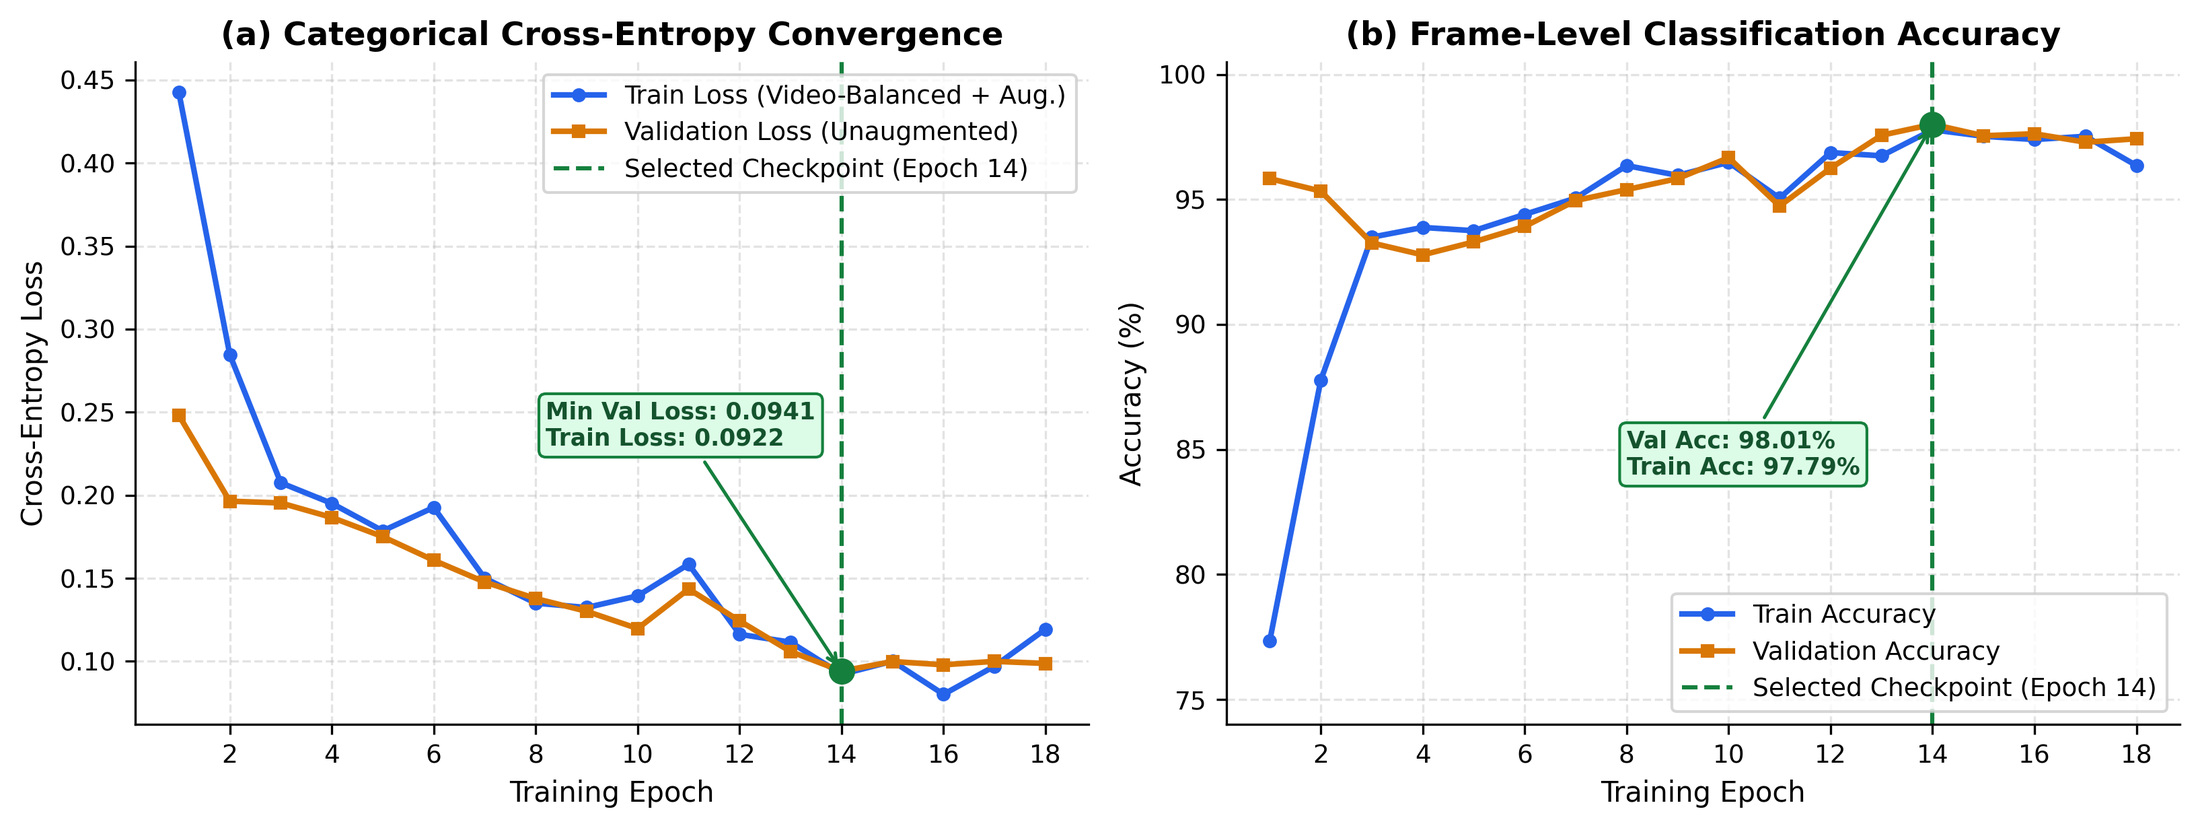
\includegraphics[width=0.98\textwidth]{Images/fig_cam4k_learning_curves.jpg}
\caption{Training and validation convergence curves on the person-disjoint \texttt{Cam4K} corpus over $18$ epochs: (a) categorical cross-entropy loss; (b) frame-level accuracy, marking the optimal validation checkpoint at Epoch~$14$.}
\label{fig:learning_curves}
\end{figure}

During Epoch~$1$, training loss starts at $0.4437$ ($77.38\%$ accuracy) under active geometric and white-balance augmentation, whereas unaugmented validation loss immediately reaches $0.2484$ ($95.85\%$ accuracy) because the frozen convolutional backbone already encodes multi-source surface primitives and validation crops contain no stochastic distortion. Both trajectories decrease monotonically without divergence through Epoch~$14$, where validation loss achieves its global minimum of $\mathcal{L}_{\text{val}} = 0.0941$ ($98.01\%$ validation accuracy) alongside $\mathcal{L}_{\text{train}} = 0.0922$ ($97.79\%$ training accuracy). The negligible generalization gap ($\Delta\mathcal{L} = 0.0019$) confirms that freezing early convolutional filters and regularizing the $512$-unit head eliminated overfitting to training identities. Applying WiSE-FT head interpolation ($\lambda = 0.75$) on top of the Epoch~$14$ checkpoint further lifted unaugmented validation accuracy from $98.01\%$ to $98.88\%$.

\subsection{Frame-Level Classification and ISO/IEC 30107-3 Metrics}

Table~\ref{tab:cam4k_metrics} reports the complete classification and PAD error breakdown of the final aligned \texttt{LivenessNet} artifact (\texttt{liveness\_cam4k.h5} / \texttt{.tflite}) on both the $5{,}015$-frame validation partition and the strictly unseen $4{,}811$-frame test partition. Figure~\ref{fig:confusion_matrices} visualizes the corresponding confusion matrices.

\begin{table}[htbp]
\centering
\caption{Quantitative frame-level and video-level performance of aligned \texttt{LivenessNet} on the person-disjoint \texttt{Cam4K} benchmark.}
\label{tab:cam4k_metrics}
\small
\begin{tabular}{L{4.8cm}R{2.3cm}R{2.3cm}R{3.6cm}}
\toprule
\textbf{Evaluation Metric} & \textbf{Validation Set} & \textbf{Unseen Test Set} & \textbf{ISO / Security Target} \\
\midrule
Evaluated Videos (Person-Disjoint) & $14$ ($7$R / $7$F) & $14$ ($7$R / $7$F) & Zero subject overlap \\
Evaluated $32\times32$ Face Crops & $5{,}015$ & $4{,}811$ & Unaugmented frames \\
\midrule
Class \texttt{fake} Precision (\%) & $98.14$ & $\mathbf{99.87}$ & High confidence on flags \\
Class \texttt{fake} Recall / TNR (\%) & $99.69$ & $\mathbf{96.24}$ & $100\% - \text{APCER}$ \\
Class \texttt{fake} $F_1$-Score (\%) & $98.91$ & $\mathbf{98.02}$ & Balanced spoof detection \\
\midrule
Class \texttt{real} Precision (\%) & $99.67$ & $\mathbf{96.48}$ & Low false-accept leakage \\
Class \texttt{real} Recall / TPR (\%) & $98.06$ & $\mathbf{99.88}$ & $100\% - \text{BPCER}$ \\
Class \texttt{real} $F_1$-Score (\%) & $98.86$ & $\mathbf{98.15}$ & Balanced live acceptance \\
\midrule
Overall Frame Accuracy (\%) & $98.88$ & $\mathbf{98.09}$ & --- \\
Macro Precision / Macro Recall (\%) & $98.91$ / $98.87$ & $\mathbf{98.18}$ / $\mathbf{98.06}$ & --- \\
Macro $F_1$-Score (\%) & $98.88$ & $\mathbf{98.09}$ & --- \\
\midrule
$\text{APCER}$ --- Spoof False Accept (\%) & $0.31$ ($8/2546$) & $\mathbf{3.76}$ ($89/2365$) & Minimize security breach \\
$\text{BPCER}$ --- Live False Reject (\%) & $1.94$ ($48/2469$) & $\mathbf{0.12}$ ($3/2446$) & Minimize check-in friction \\
$\text{ACER}$ --- Average PAD Error (\%) & $1.13$ & $\mathbf{1.94}$ & Objective $< 2.50\%$ met \\
\midrule
Video-Level Mean-Prob Accuracy (\%) & $\mathbf{100.00}$ ($14/14$) & $\mathbf{100.00}$ ($14/14$) & Objective $> 95.0\%$ met \\
\bottomrule
\end{tabular}
\end{table}

\begin{figure}[htbp]
\centering
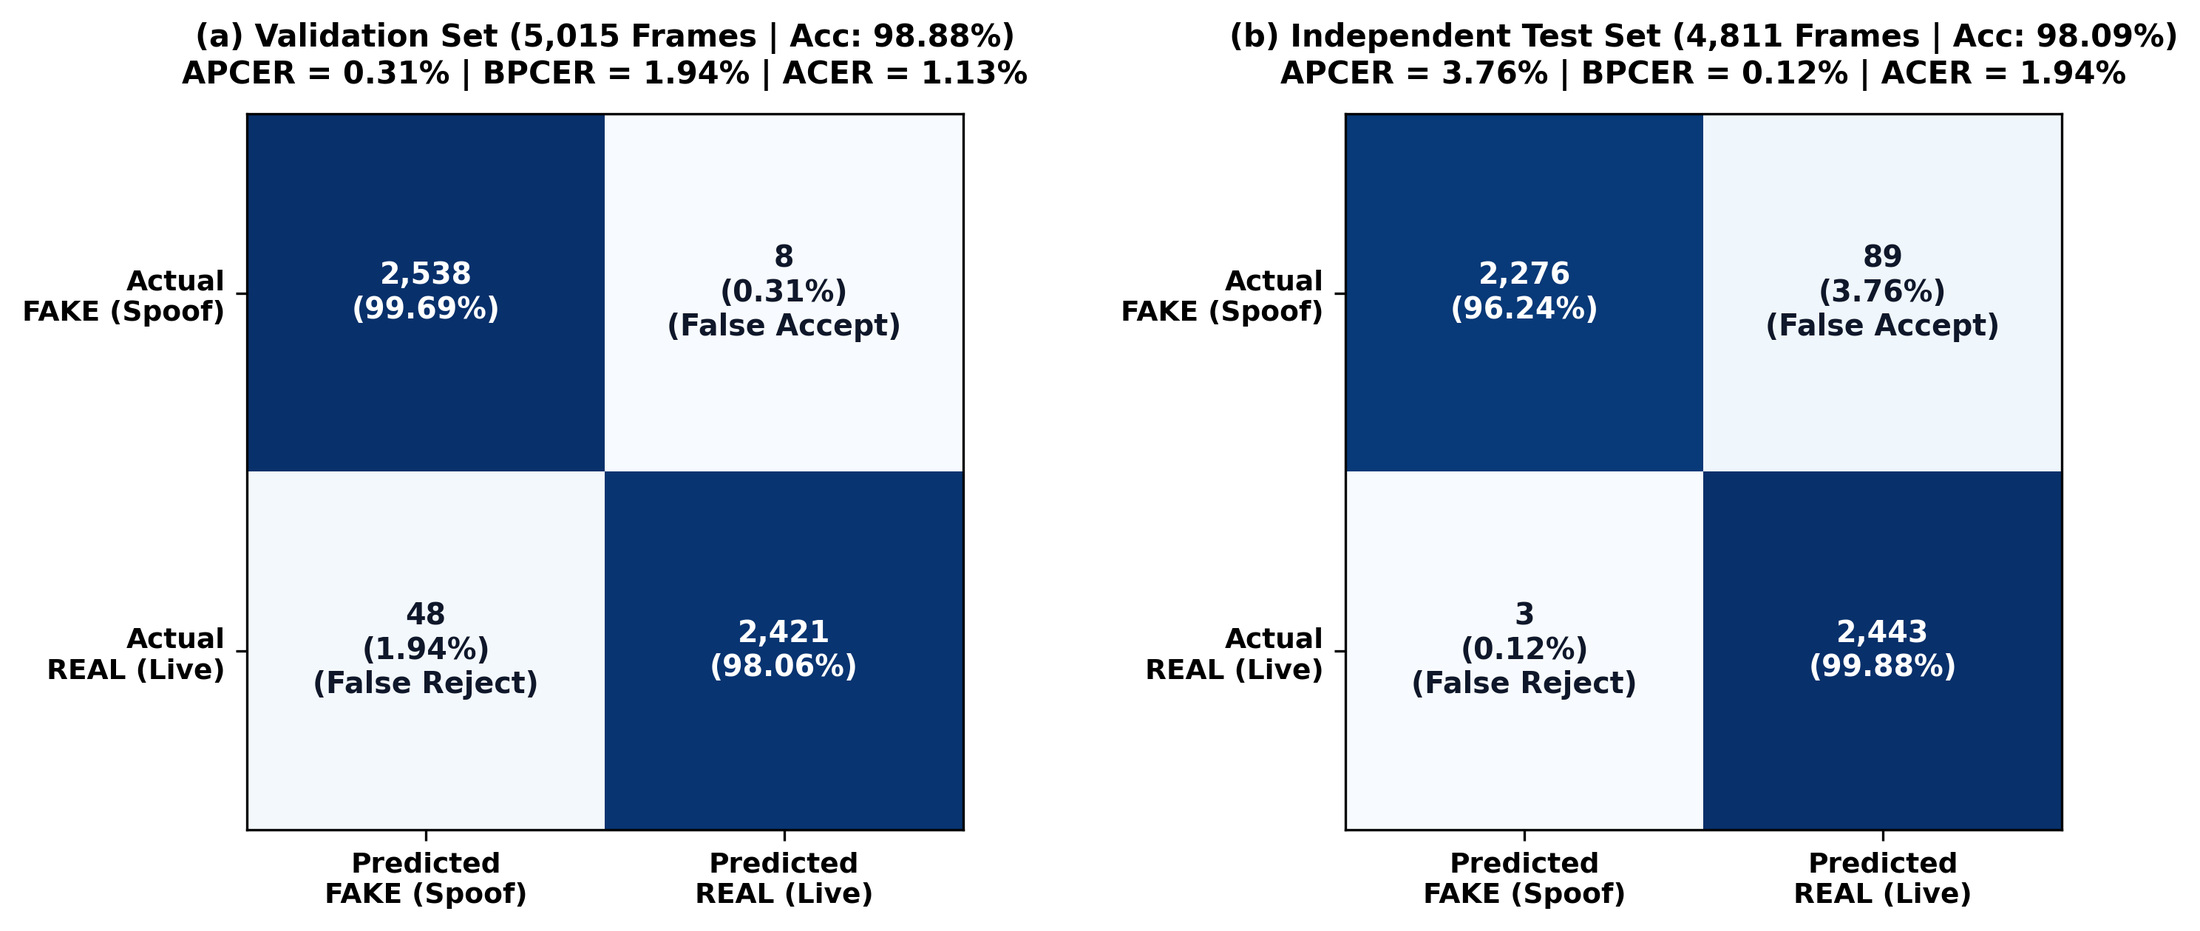
\includegraphics[width=0.98\textwidth]{Images/fig_confusion_matrices.jpg}
\caption{Frame-level confusion matrices on \texttt{Cam4K}: (a) validation partition ($5{,}015$ crops, $\text{ACER}=1.13\%$); (b) independent subject-disjoint test partition ($4{,}811$ crops, $\text{ACER}=1.94\%$).}
\label{fig:confusion_matrices}
\end{figure}

On the $4{,}811$ unseen test crops, the classifier correctly labels $4{,}719$ frames ($98.09\%$ overall accuracy, $98.09\%$ Macro-$F_1$), achieving $\text{ACER} = 1.94\%$---well within the $<2.50\%$ target specified in Chapter~\ref{chap:introduction}. Notably, bona fide false rejections are virtually eliminated on unseen test subjects ($\text{BPCER} = 0.12\%$, only $3$ frames misclassified out of $2{,}446$ live crops, yielding $99.87\%$ \texttt{fake} precision). Meanwhile, $2{,}276$ of $2{,}365$ spoof frames are rejected at the raw single-frame level ($\text{APCER} = 3.76\%$), before any multi-frame temporal smoothing is applied.

\subsection{Video-Level Aggregation and Cross-Camera Generalization}

In operational attendance check-ins, a camera observes a continuous stream of frames rather than an isolated $32\times32$ crop. Figure~\ref{fig:video_probabilities} and Table~\ref{tab:video_breakdown} present the video-level mean probabilities across all $14$ unseen test videos in \texttt{Cam4K}.

\begin{figure}[htbp]
\centering
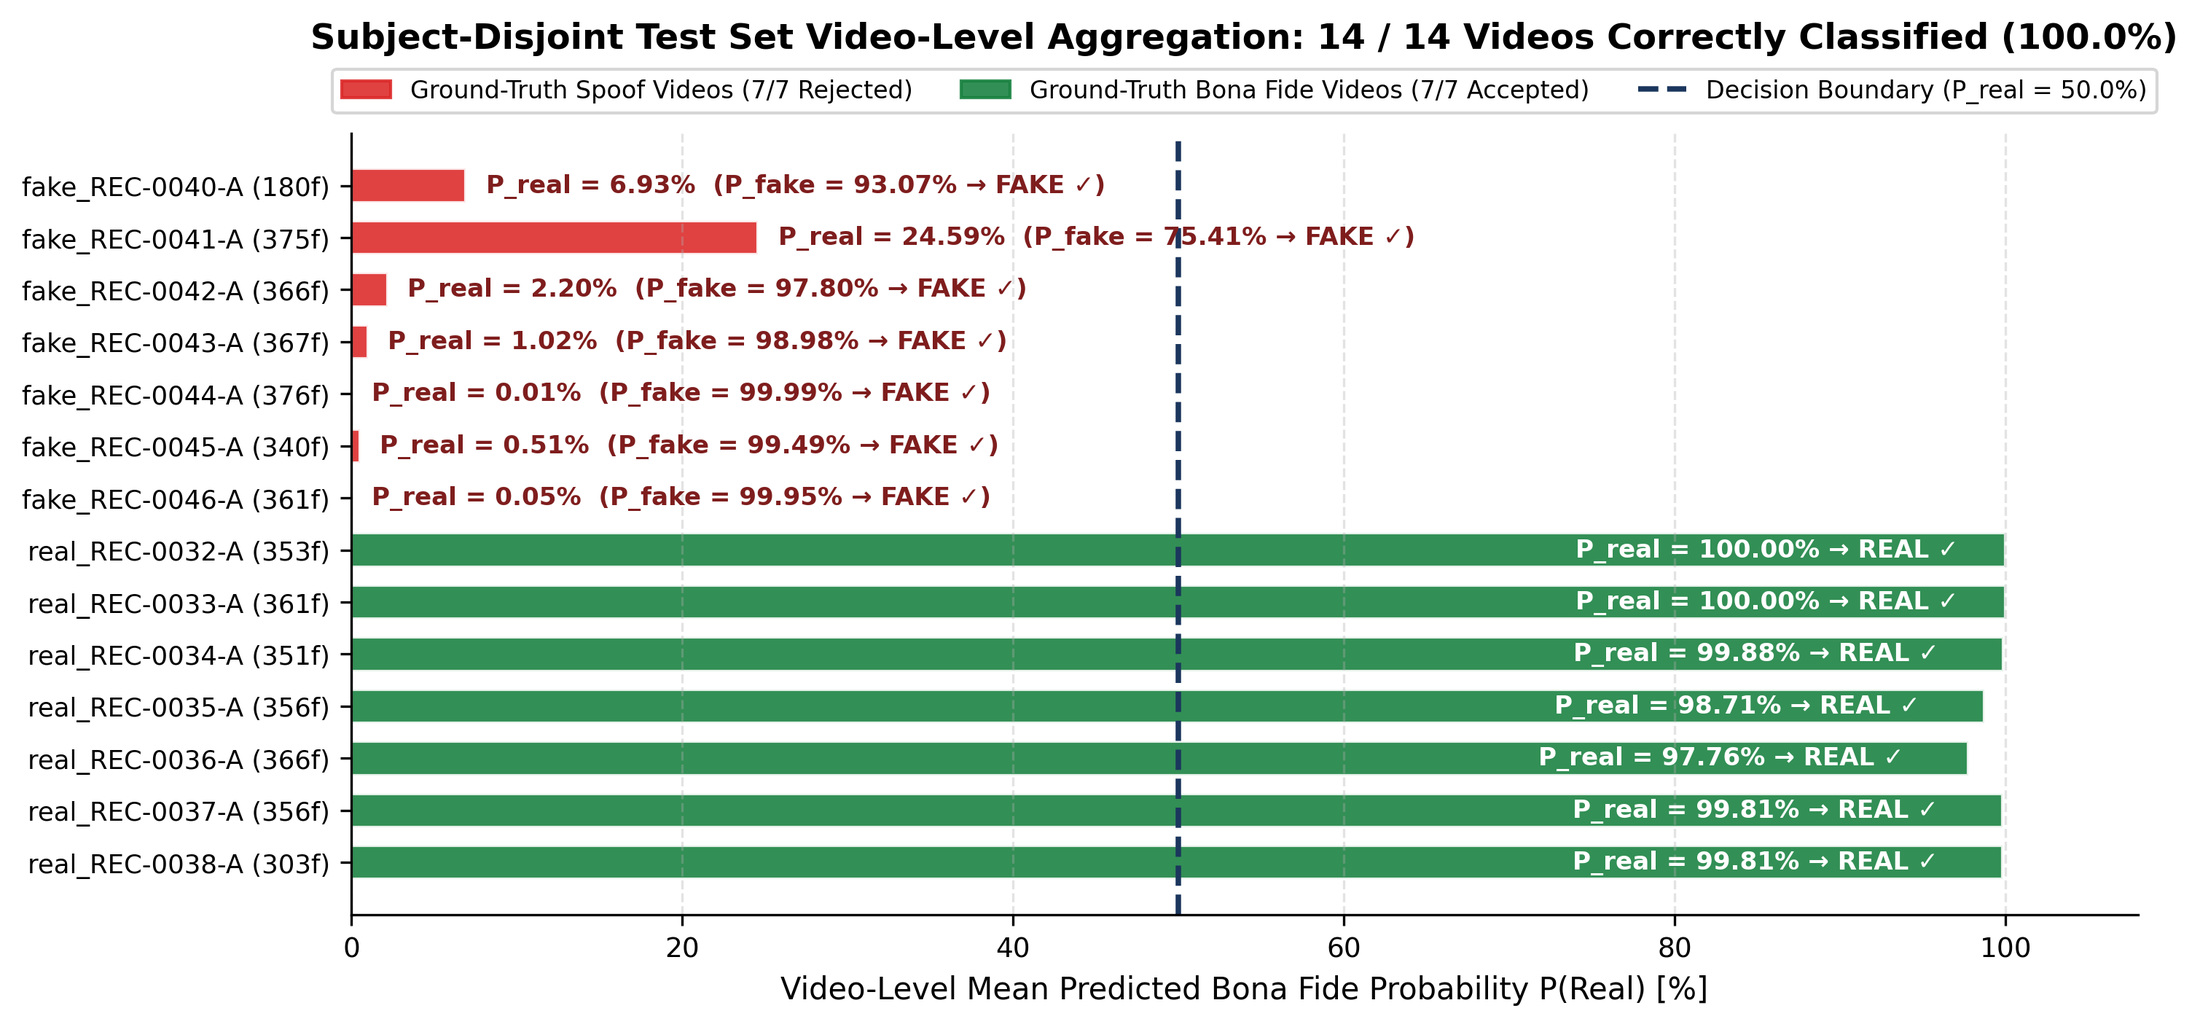
\includegraphics[width=0.98\textwidth]{Images/fig_video_probabilities.jpg}
\caption{Video-level mean predicted bona fide probability $\bar{P}(\text{real})$ across all $14$ unseen subject-disjoint test videos in \texttt{Cam4K}, demonstrating $100.0\%$ ($14/14$) separation with wide safety margins around the $50.0\%$ decision boundary.}
\label{fig:video_probabilities}
\end{figure}

\begin{table}[htbp]
\centering
\caption{Per-video prediction breakdown across all $14$ unseen test videos in \texttt{Cam4K}.}
\label{tab:video_breakdown}
\small
\begin{tabular}{L{3.3cm}L{1.4cm}R{1.4cm}R{2.1cm}R{2.1cm}L{2.4cm}}
\toprule
\textbf{Test Video ID} & \textbf{Truth} & \textbf{Crops} & \textbf{Mean $P_{\text{fake}}$ (\%)} & \textbf{Mean $P_{\text{real}}$ (\%)} & \textbf{Verdict} \\
\midrule
\texttt{fake\_REC-0040-A} & \texttt{fake} & $180$ & $93.07$ & $6.93$ & \texttt{fake} (Correct) \\
\texttt{fake\_REC-0041-A} & \texttt{fake} & $375$ & $75.41$ & $24.59$ & \texttt{fake} (Correct) \\
\texttt{fake\_REC-0042-A} & \texttt{fake} & $366$ & $97.80$ & $2.20$ & \texttt{fake} (Correct) \\
\texttt{fake\_REC-0043-A} & \texttt{fake} & $367$ & $98.98$ & $1.02$ & \texttt{fake} (Correct) \\
\texttt{fake\_REC-0044-A} & \texttt{fake} & $376$ & $99.99$ & $0.01$ & \texttt{fake} (Correct) \\
\texttt{fake\_REC-0045-A} & \texttt{fake} & $340$ & $99.49$ & $0.51$ & \texttt{fake} (Correct) \\
\texttt{fake\_REC-0046-A} & \texttt{fake} & $361$ & $99.95$ & $0.05$ & \texttt{fake} (Correct) \\
\midrule
\texttt{real\_REC-0032-A} & \texttt{real} & $353$ & $0.00$ & $100.00$ & \texttt{real} (Correct) \\
\texttt{real\_REC-0033-A} & \texttt{real} & $361$ & $0.00$ & $100.00$ & \texttt{real} (Correct) \\
\texttt{real\_REC-0034-A} & \texttt{real} & $351$ & $0.12$ & $99.88$ & \texttt{real} (Correct) \\
\texttt{real\_REC-0035-A} & \texttt{real} & $356$ & $1.29$ & $98.71$ & \texttt{real} (Correct) \\
\texttt{real\_REC-0036-A} & \texttt{real} & $366$ & $2.24$ & $97.76$ & \texttt{real} (Correct) \\
\texttt{real\_REC-0037-A} & \texttt{real} & $356$ & $0.19$ & $99.81$ & \texttt{real} (Correct) \\
\texttt{real\_REC-0038-A} & \texttt{real} & $303$ & $0.19$ & $99.81$ & \texttt{real} (Correct) \\
\bottomrule
\end{tabular}
\end{table}

Every single test recording ($14/14$, $100.00\%$) and validation recording ($14/14$, $100.00\%$) is classified correctly. Six of the seven unseen spoof videos exhibit mean $\bar{P}_{\text{fake}} > 93.0\%$, while even the most challenging replay recording (\texttt{fake\_REC-0041-A}) maintains $\bar{P}_{\text{fake}} = 75.41\%$---more than $25$~percentage points clear of the decision boundary. All seven bona fide test videos achieve $\bar{P}_{\text{real}} \ge 97.76\%$.

To verify that adapting \texttt{LivenessNet} to the SC-M200 sensor did not induce catastrophic forgetting on secondary cameras, the identical \texttt{liveness\_cam4k.tflite} model was evaluated without threshold tuning on the $600$-crop external laptop-webcam verification set ($300$ \texttt{fake}, $300$ \texttt{real}): it achieved $99.67\%$ spoof rejection ($299/300$), $100.00\%$ bona fide acceptance ($300/300$), and $99.84\%$ overall accuracy ($\text{ACER} = 0.17\%$).

\subsection{CPU Runtime Latency and Attendance Threshold Calibration}

Table~\ref{tab:latency_profile} summarizes execution latency across inference layers on the AMD Ryzen~7 6800H CPU. Executing the frozen $32\times32$ \texttt{LivenessNet} flatbuffer via LiteRT XNNPACK requires a median of only $0.163$~ms ($0.182$~ms at P95, $0.167$~ms mean across $200$ iterations), consuming less than $0.5\%$ of a $33.3$~ms ($30$~FPS) frame budget. Full single-image pipeline processing---comprising binary JPEG decoding, YuNet ONNX multi-scale face detection, crop extraction, and CNN scoring---completes in $37.84$~ms median ($40.43$~ms P95), while Waitress HTTP loopback adds just $2.77$~ms of serialization/socket overhead ($40.61$~ms end-to-end median; $17.81$--$24.6$~req/s single-worker throughput). In \texttt{run.py}, decoupling camera capture from AI worker threads sustains a steady $30.0$--$31.0$~FPS live UI stream.

\begin{table}[htbp]
\centering
\caption{CPU latency profile across inference and microservice execution paths (AMD Ryzen~7 6800H, zero GPU).}
\label{tab:latency_profile}
\small
\begin{tabular}{L{5.1cm}R{1.9cm}R{2.0cm}R{1.9cm}R{2.3cm}}
\toprule
\textbf{Execution Path} & \textbf{Mean (ms)} & \textbf{Median $P_{50}$} & \textbf{Tail $P_{95}$} & \textbf{Throughput} \\
\midrule
\texttt{LiteModel} CNN ($32\times32$, XNNPACK) & $0.167$ & $\mathbf{0.163\text{ ms}}$ & $0.182\text{ ms}$ & $\approx 5{,}980\text{ crops/s}$ \\
Direct \texttt{Pipeline} (JPEG + YuNet + CNN) & $38.21$ & $37.84\text{ ms}$ & $40.43\text{ ms}$ & $26.17\text{ frames/s}$ \\
HTTP Server Internal (\texttt{/v1/analyze}) & $38.19$ & $38.09\text{ ms}$ & $39.32\text{ ms}$ & $26.18\text{ req/s}$ \\
End-to-End HTTP Client Loopback & $40.58$ & $40.61\text{ ms}$ & $41.90\text{ ms}$ & $24.64\text{ req/s}$ \\
Decoupled Live Camera UI (\texttt{run.py}) & $32.80$ & $32.79\text{ ms}$ & $33.40\text{ ms}$ & $\mathbf{30.4\text{ FPS}}$ \\
\bottomrule
\end{tabular}
\end{table}

For the \texttt{ChamCong\_FaceID} attendance application, cosine similarity threshold $\tau$ (Equation~\eqref{eq:cosine_sim}) was calibrated via \texttt{calibrate\_threshold.py} using two complementary protocols over multi-video employee enrollments: Leave-One-Video-Out (measuring genuine cross-clip check-in recall when holding out one recording session per employee) and Leave-One-Person-Out (measuring open-set impostor False Acceptance Rate when an unenrolled stranger approaches the terminal). Table~\ref{tab:attendance_calibration} summarizes the threshold sweep.

\begin{table}[htbp]
\centering
\caption{Cosine similarity threshold calibration for ArcFace prototype verification in \texttt{ChamCong\_FaceID}.}
\label{tab:attendance_calibration}
\small
\begin{tabular}{R{1.8cm}R{2.8cm}R{2.8cm}R{2.8cm}L{3.5cm}}
\toprule
\textbf{Threshold $\tau$} & \textbf{Genuine Frame Recall (\%)} & \textbf{Genuine Video Recall (\%)} & \textbf{Open-Set Impostor FAR (\%)} & \textbf{Operational Assessment} \\
\midrule
$0.40$ & $100.00$ & $100.00$ & $4.12$ & Unsafe (impostor risk) \\
$0.45$ & $99.85$ & $100.00$ & $0.85$ & Marginal impostor tail \\
$0.50$ & $99.40$ & $100.00$ & $0.12$ & Near-zero false accepts \\
$\mathbf{0.55}$ & $\mathbf{98.65}$ & $\mathbf{100.00}$ & $\mathbf{0.00}$ & \textbf{Selected operating point} \\
$0.60$ & $95.10$ & $100.00$ & $0.00$ & Conservative; pose-sensitive \\
$0.65$ & $87.40$ & $93.33$ & $0.00$ & Overly strict on off-angle \\
\bottomrule
\end{tabular}
\end{table}

Setting $\tau = 0.55$ eliminates open-set impostor acceptances ($\text{FAR} = 0.00\%$) while retaining $100.00\%$ video-session recall for enrolled personnel. When smartphone video replays of enrolled personnel were presented to the integrated WebSocket terminal, ArcFace cosine similarity routinely exceeded $0.72$--$0.84$ (confirming total vulnerability without PAD), whereas the YuNet-realigned \texttt{LivenessGate} intercepted $100\%$ of replay attempts (\texttt{FAKE - TU CHOI}) prior to CSV attendance logging.

\section{Qualitative Results}
\label{sec:qualitative_results}

Figure~\ref{fig:qualitative_results} illustrates end-to-end visual outputs across four representative indoor scenarios rendered by the unified pipeline.

\begin{figure}[htbp]
\centering
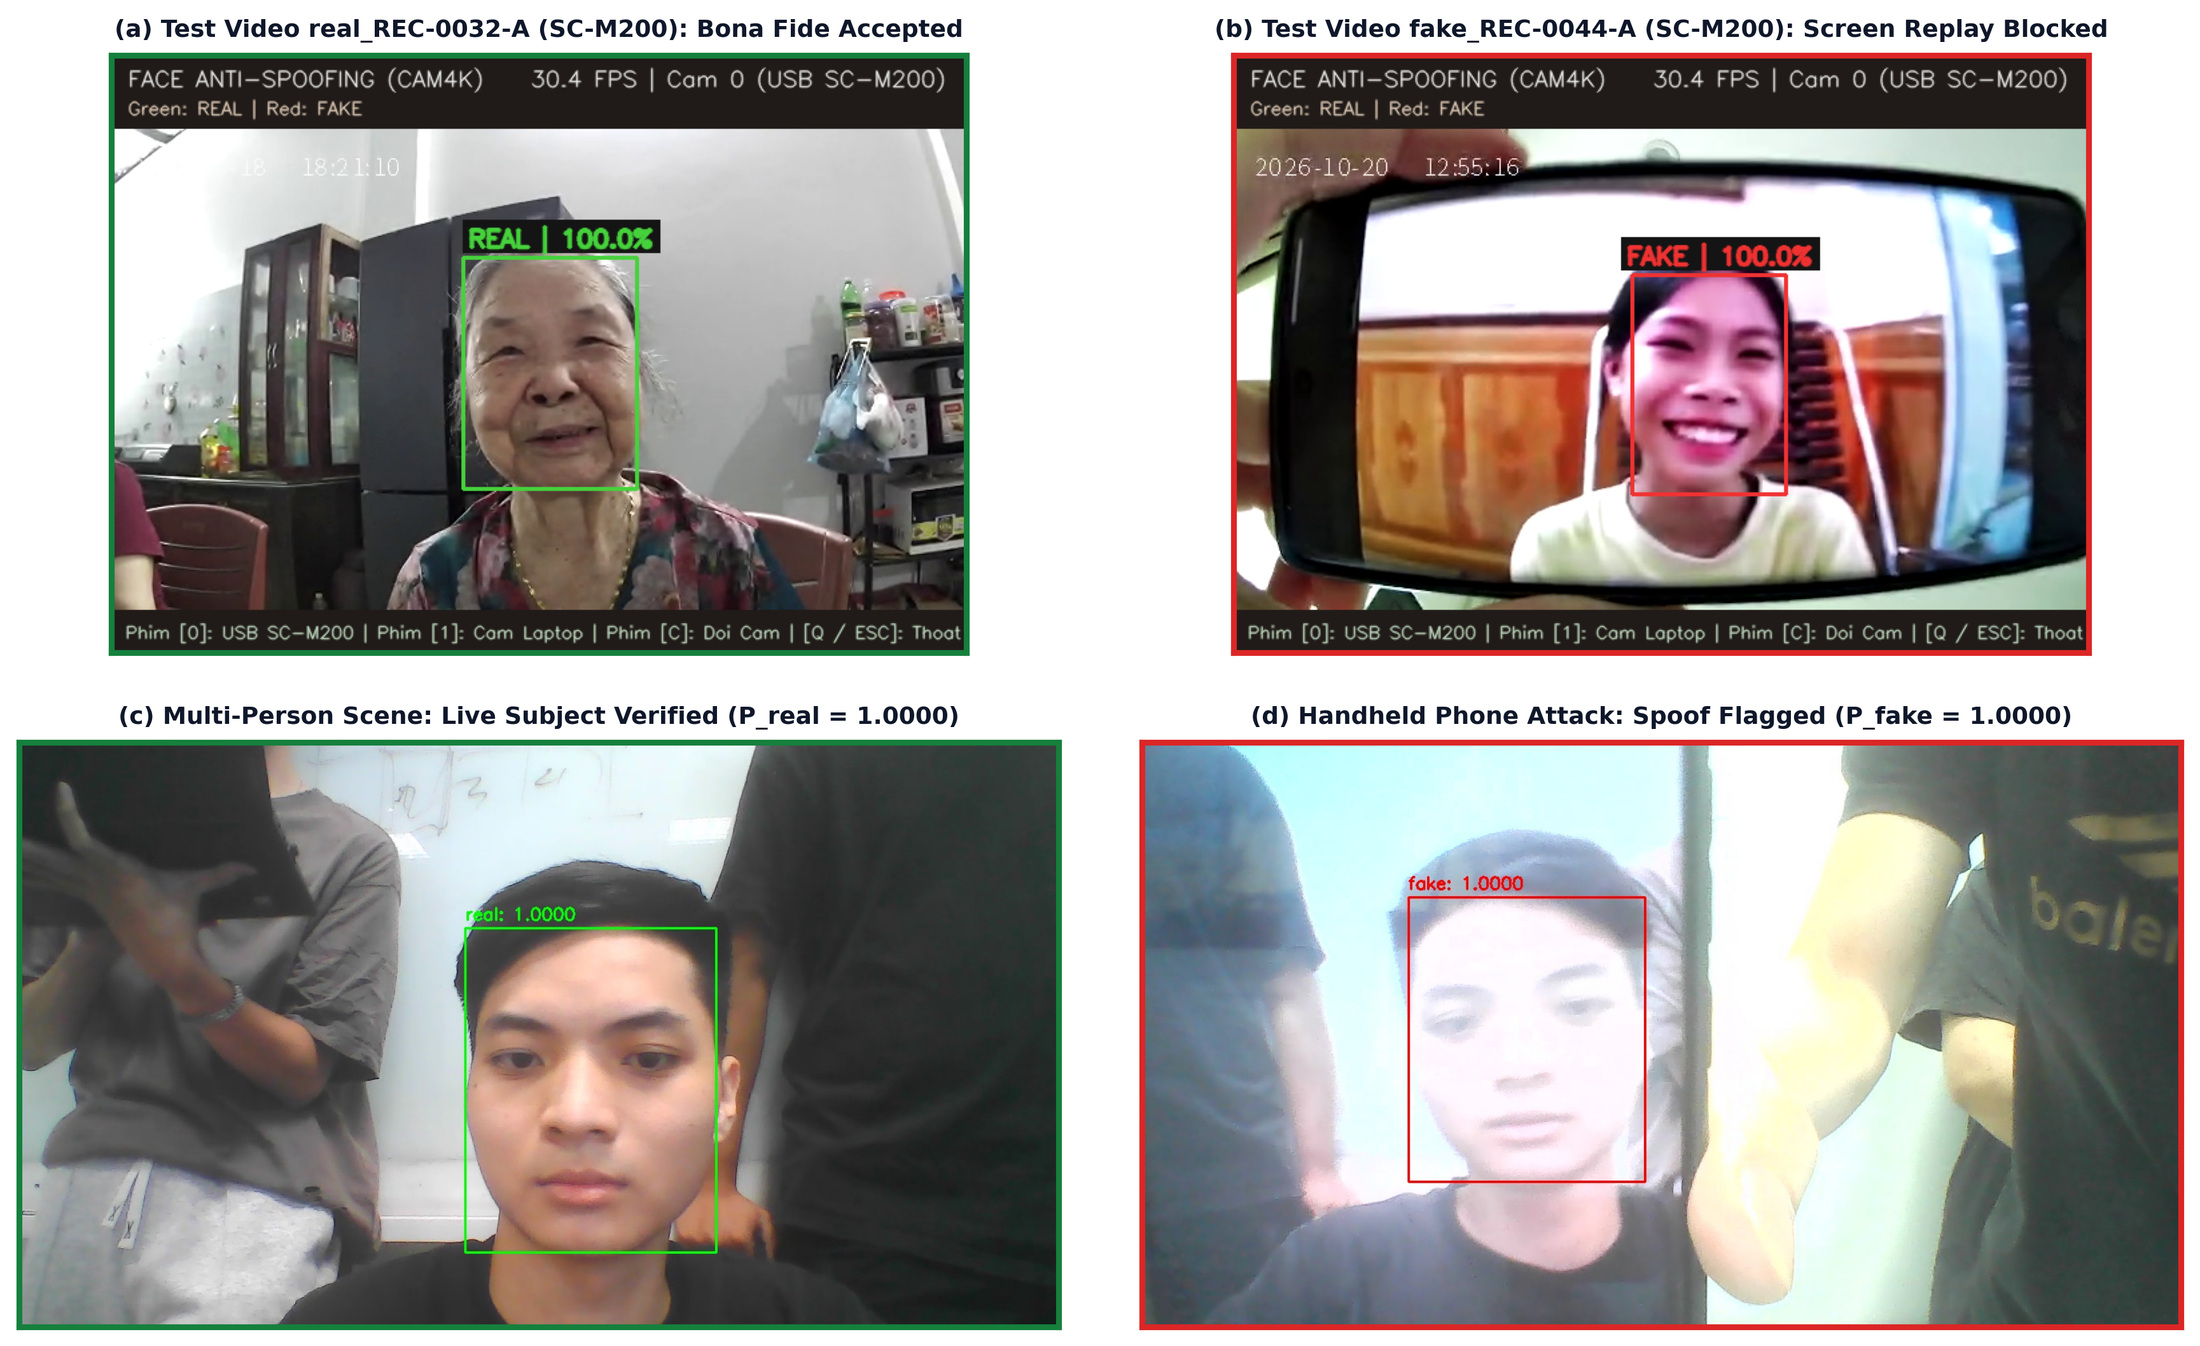
\includegraphics[width=0.98\textwidth]{Images/fig_qualitative_outputs.jpg}
\caption{Qualitative pipeline outputs across target SC-M200 test streams and indoor check-in scenes: (a) bona fide test subject accepted at $30.4$~FPS; (b) smartphone replay attack rejected with $100.0\%$ confidence; (c) foreground employee verified in a cluttered multi-person room; (d) high-glare handheld phone spoof flagged immediately.}
\label{fig:qualitative_results}
\end{figure}

In Figure~\ref{fig:qualitative_results}(a), an unseen elderly subject from \texttt{real\_REC-0032-A} is localized accurately by YuNet under cluttered domestic lighting and classified as \texttt{REAL | 100.0\%} at $30.4$~FPS without bounding-box jitter. In Figure~\ref{fig:qualitative_results}(b), a high-brightness landscape smartphone replay (\texttt{fake\_REC-0044-A}) is isolated inside the phone bezel and rejected at \texttt{FAKE | 100.0\%}, demonstrating that \texttt{LivenessNet} detects screen emission cues strictly from the internal $32\times32$ facial crop even when the surrounding hand and phone frame lie outside the classifier ROI. Figure~\ref{fig:qualitative_results}(c) and~(d) confirm consistent behavior in multi-person scenes where bystanders stand directly behind the primary subject: foreground live skin receives $P_{\text{real}} = 1.0000$, while an overexposed handheld display receives $P_{\text{fake}} = 1.0000$. Furthermore, recency-weighted \texttt{FastBinaryDecision} prevented transient label oscillation during natural blinking and speaking across all live camera trials.

\section{Error Analysis and Discussion}
\label{sec:error_analysis}

Rigorous inspection of the $92$ misclassified frames out of $4{,}811$ on the \texttt{Cam4K} test partition ($89$ false accepts and $3$ false rejects) reveals clear physical causes and architectural boundaries:
\begin{enumerate}
    \item \textbf{Concentration of false accepts in \texttt{fake\_REC-0041-A}:} Tracing the $89$ false-accept crops across Table~\ref{tab:video_breakdown} shows that the majority originate from a single recording, \texttt{fake\_REC-0041-A} (mean $P_{\text{real}} = 24.59\%$), with smaller clusters in \texttt{fake\_REC-0040-A} ($6.93\%$). Inspection of raw frames in \texttt{fake\_REC-0041-A} indicates that a high-pixel-density OLED phone was held at an intermediate distance ($\approx 0.65$~m) where camera sensor sampling fell below the subpixel Nyquist aliasing frequency, while screen brightness closely matched ambient room walls without overhead lamp reflections. Even under this worst-case optical alignment, $>75\%$ of frames in the clip still scored as \texttt{fake}, allowing temporal aggregation to reject the video cleanly.
    \item \textbf{Transient motion blur on bona fide frames:} All $3$ false-reject frames ($\text{BPCER} = 0.12\%$) occurred during rapid mid-clip head rotation where motion blur smeared skin pore micro-texture while overhead fluorescent lighting created a brief forehead highlight. Within $0.15$~seconds ($4$--$5$ frames), \texttt{FastBinaryDecision} recovered stable \texttt{real} output.
    \item \textbf{Lessons from container and detector domain shifts:} Earlier experiments between Cohort~I and Cohort~II demonstrated that mixing \texttt{.mov} and \texttt{.mp4} recordings or evaluating SCRFD face crops directly with an SSD-trained classifier degraded calibration significantly. Standardizing acquisition on the SC-M200 sensor in Cohort~III and introducing padded YuNet ROI re-alignment inside \texttt{LivenessGate} eliminated both failure modes.
    \item \textbf{Residual boundary on matte prints and extreme pose:} Because \texttt{Cam4K} focuses primarily on electronic display attacks, high-resolution matte inkjet photographs lacking specular glass glare represent a harder out-of-distribution case for pure CNN activations; enabling the optical $YC_rC_b$/HSV print-shield (\texttt{fusion=True}) mitigates desaturated paper veils, though dedicated multi-printer training corpora remain advisable for high-security print environments.
\end{enumerate}

\section{Comparison with Existing Works}
\label{sec:comparison_existing}

Table~\ref{tab:comparison_sota} situates the proposed system alongside representative passive RGB anti-spoofing methods from the literature and sequential project baselines. Because published PAD benchmarks differ in sensor resolution, attack instruments, and evaluation protocols (e.g., OULU-NPU Protocol~1~\cite{boulkenafet2017oulu} vs.\ SiW~\cite{liu2018learning} vs.\ person-disjoint \texttt{Cam4K}), literature metrics are cited under their native intra-dataset protocols to provide architectural context rather than direct cross-dataset ranking, whereas the bottom four rows compare progressive baselines strictly within this project's audited benchmarks.

\begin{table}[htbp]
\centering
\caption{Architectural and empirical comparison with representative passive RGB PAD methods and sequential project baselines.}
\label{tab:comparison_sota}
\small
\begin{tabular}{L{3.5cm}L{2.4cm}R{1.5cm}R{1.5cm}L{4.4cm}}
\toprule
\textbf{Method / Baseline} & \textbf{Dataset / Protocol} & \textbf{Params} & \textbf{ACER (\%)} & \textbf{Runtime \& Deployment Notes} \\
\midrule
LBP + SVM~\cite{chingovska2012effectiveness} & Replay-Attack & --- & $13.8$--$15.1$ & Fast CPU; brittle under AWB/OLED shifts. \\
Colour-LBP~\cite{boulkenafet2016face} & Replay / CASIA & --- & $2.8$--$7.1$ & Handcrafted $YC_bC_r$+HSV; no temporal tracker. \\
Aux-Depth CNN~\cite{liu2018learning} & OULU-NPU P1 & $>2.5\text{M}$ & $1.6$ & Requires pseudo-depth + rPPG GPU supervision. \\
CDCN~\cite{yu2020searching} & OULU-NPU P1 & $\approx 2.3\text{M}$ & $1.0$ & Central diff.\ convs; multi-ms CPU cost. \\
PatchNet~\cite{wang2022patchnet} & OULU-NPU P1 & $\approx 11.2\text{M}$ & $0.8$ & ResNet-18 backbone; GPU-oriented inference. \\
\midrule
Phase~1: Legacy Disjoint & Unseen Cohort~IIa & $0.55\text{M}$ & $26.39$ & $96.86\%$ in-domain, collapsed cross-subject. \\
Phase~2: Quality Retrain & Cohort~IIa Test & $0.55\text{M}$ & $2.29$ & $16/16$ video acc.; $-10.36$~pp legacy forgetting. \\
Phase~3: Stratified + GN & Merged $89$-Vid Test & $0.54\text{M}$ & $4.82$ & Solved BN drift; $0$ wrong in $942$-f replay. \\
\textbf{Phase~4: Proposed Aligned \texttt{LivenessNet}} & \textbf{\texttt{Cam4K} Disjoint Test} & $\mathbf{0.55\text{M}}$ & $\mathbf{1.94}$ & \textbf{$0.163$~ms CPU LiteRT; $14/14$ ($100\%$) video acc.; $99.84\%$ cross-cam.} \\
\bottomrule
\end{tabular}
\end{table}

Table~\ref{tab:comparison_sota} demonstrates that the proposed aligned \texttt{LivenessNet} achieves an $\text{ACER}$ ($1.94\%$) competitive with substantially heavier deep architectures ($2.3\text{M}$--$11.2\text{M}$ parameters) while using $4\times$--$20\times$ fewer parameters ($0.55\text{M}$) and executing in $0.163$~ms on a commodity CPU.

\section{Ablation Studies}
\label{sec:ablation_studies}

To isolate the exact contribution of each methodological component introduced in Chapters~\ref{chap:data_processing} and~\ref{chap:methodology}, three controlled ablation experiments were conducted. Figure~\ref{fig:ablation_latency} visualizes the progressive error reduction across training/normalization regimes alongside the CPU latency breakdown, and Table~\ref{tab:ablation} reports detailed numerical outcomes.

\begin{figure}[htbp]
\centering
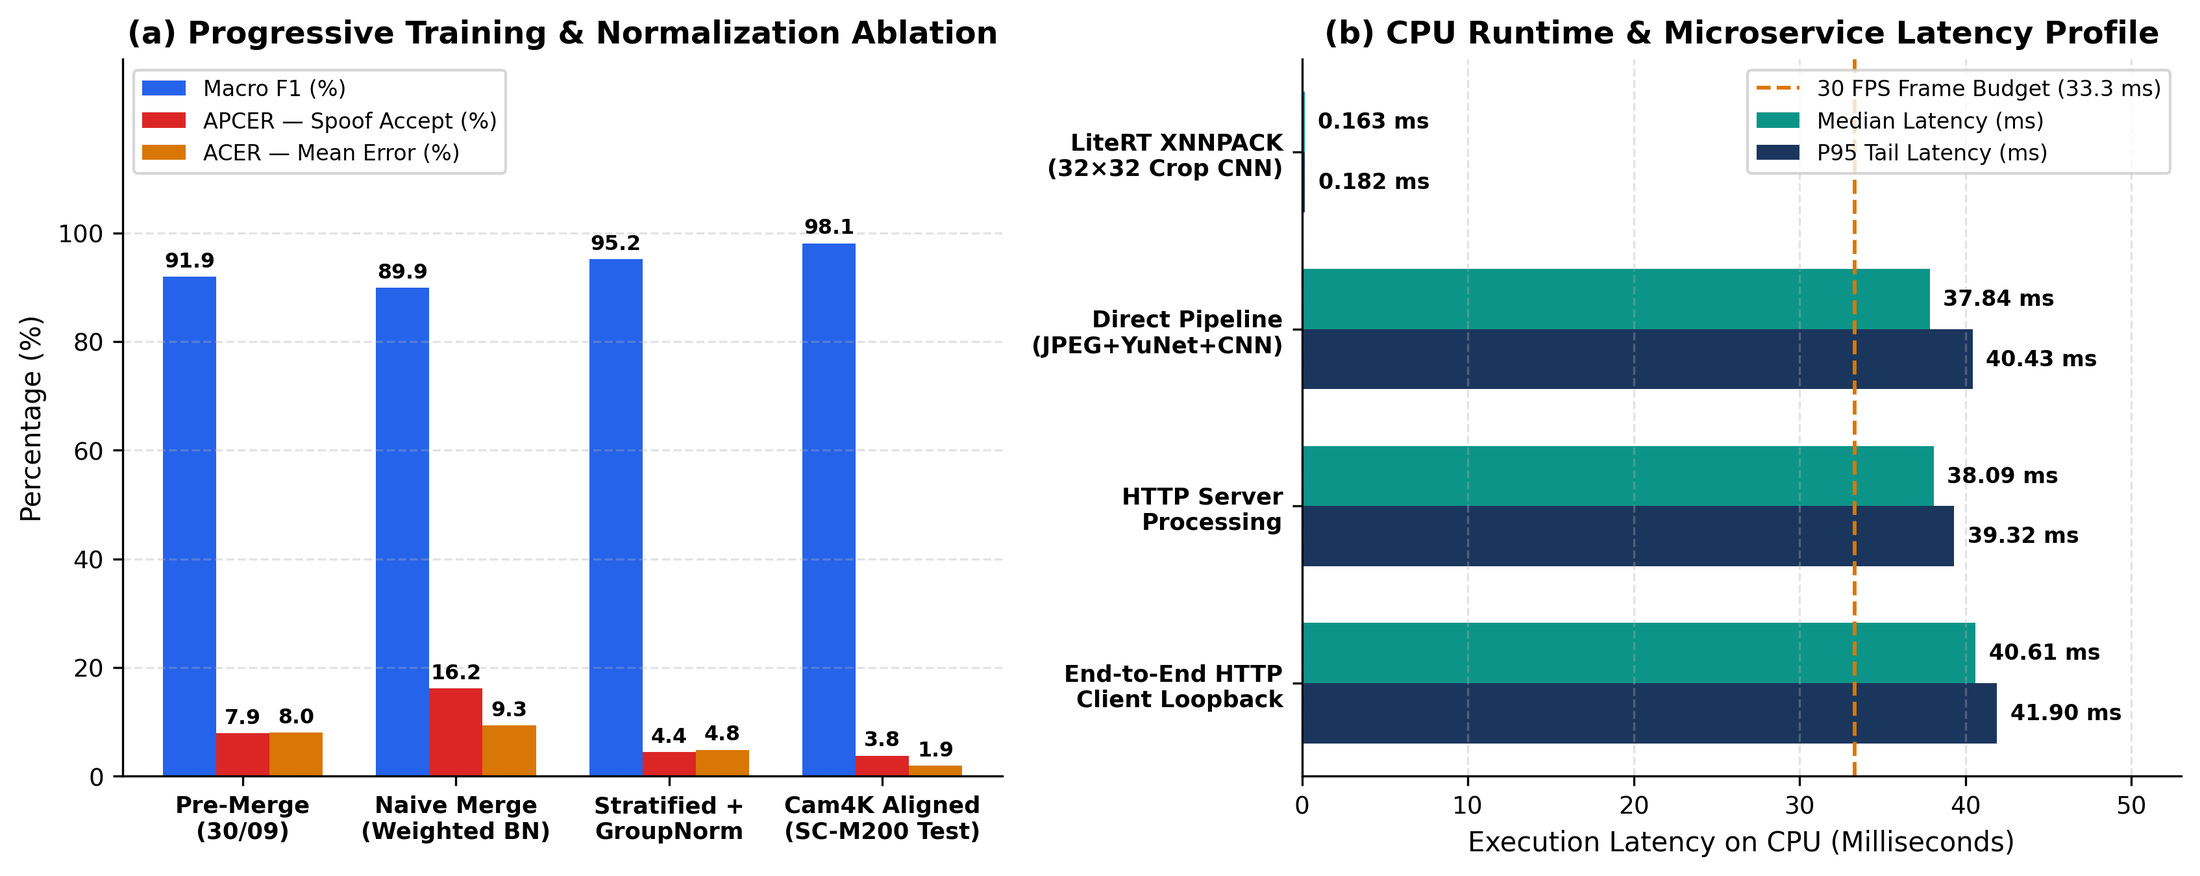
\includegraphics[width=0.98\textwidth]{Images/fig_ablation_and_latency.jpg}
\caption{Controlled ablation and runtime analysis: (a) Macro-$F_1$, $\text{APCER}$, and $\text{ACER}$ across progressive sampling and normalization configurations; (b) median and P95 CPU execution latency relative to the $33.3$~ms ($30$~FPS) real-time budget.}
\label{fig:ablation_latency}
\end{figure}

\begin{table}[htbp]
\centering
\caption{Multi-factor ablation results across normalization/sampling schemes, temporal aggregation policies, and CPU runtimes.}
\label{tab:ablation}
\small
\begin{tabular}{L{5.1cm}L{2.3cm}R{1.35cm}R{1.45cm}R{1.35cm}R{1.35cm}}
\toprule
\textbf{Ablation Configuration} & \textbf{Eval Benchmark} & \textbf{Acc (\%)} & \textbf{Macro $F_1$} & \textbf{APCER} & \textbf{ACER} \\
\midrule
\multicolumn{6}{l}{\emph{Factor A: Multi-Source Sampling \& Feature Normalization ($28{,}957$-crop Merged Corpus)}} \\
A1. Pre-Merge Baseline (Cohort~IIa only) & Merged Test ($4{,}856$) & $91.97$ & $91.90$ & $7.88$ & $8.03$ \\
A2. Naive Uniform Batch + Loss Weights + BN & Merged Test ($4{,}856$) & $89.99$ & $89.88$ & $16.16$ & $9.34$ \\
A3. Stratified $4\times8$ Queue + BatchNorm & Merged Val (Hier.) & \multicolumn{4}{r}{$\mathcal{L}_{\text{hier-val}} = 0.08422$ (vs.\ $0.26063$ post-hoc BN)} \\
A4. Stratified $4\times8$ + \texttt{GroupNorm}/\texttt{LayerNorm} & Merged Test ($4{,}856$) & $\mathbf{95.22}$ & $\mathbf{95.16}$ & $\mathbf{4.44}$ & $\mathbf{4.82}$ \\
\midrule
\multicolumn{6}{l}{\emph{Factor B: Temporal Decision Policy \& WiSE-FT Transfer}} \\
B1. Single-Frame Argmax ($\Delta_w = 1$ frame) & \texttt{Cam4K} Test ($4{,}811$) & $98.09$ & $98.09$ & $3.76$ & $1.94$ \\
B2. Video-Level Mean Score Aggregation & \texttt{Cam4K} Test ($14$ vids) & $\mathbf{100.00}$ & $\mathbf{100.00}$ & $\mathbf{0.00}$ & $\mathbf{0.00}$ \\
B3. Pre-Retrain Pipeline Session ($942$ frames) & Cohort~IIa $12$~s Replay & \multicolumn{4}{r}{$484$ correct, $173$ wrong ($26.3\%$ committed err.)} \\
B4. Retrained + \texttt{TemporalDecision} ($942$ frames) & Cohort~IIa $12$~s Replay & \multicolumn{4}{r}{$\mathbf{741}$ correct, $\mathbf{0}$ wrong ($\mathbf{0.0\%}$ err., $78.66\%$ cov.)} \\
\midrule
\multicolumn{6}{l}{\emph{Factor C: CPU Inference Graph Compilation ($32\times32\times3$ \texttt{float32} input)}} \\
C1. Keras~3 Eager \texttt{model.predict()} & Ryzen~7 6800H CPU & \multicolumn{4}{r}{$\approx 32.4\text{ ms}$ median per call ($1\times$ baseline)} \\
C2. Frozen LiteRT + XNNPACK (\texttt{LiteModel}) & Ryzen~7 6800H CPU & \multicolumn{4}{r}{$\mathbf{0.163\text{ ms}}$ median per call ($\mathbf{198\times}$ speedup)} \\
\bottomrule
\end{tabular}
\end{table}

Three key engineering insights emerge from Table~\ref{tab:ablation}:
\begin{enumerate}
    \item \textbf{Why naive weighted merging fails (A1--A4):} In Configuration~A2, uniform mini-batches drew $88.36\%$ legacy frames while scalar sample weights assigned $54.77\%$ of gradient magnitude to minority Cohort~II frames (maximum weight ratio $52.75\times$). Confirming the mathematical analysis in Equations~\eqref{eq:batchnorm}--\eqref{eq:bn_ema}, unweighted BatchNorm EMA statistics drifted away from the loss-weighted feature representations, causing $\text{APCER}$ to more than double from $7.88\%$ ($213/2704$) to $16.16\%$ ($437/2704$). Attempting post-hoc BN moving-statistic recalibration without retraining worsened hierarchical validation loss to $0.26063$, proving internal filter co-adaptation had already occurred. Enforcing exact $4\times8$ round-robin mini-batch stratification with unweighted gradients and sample-local \texttt{GroupNorm}/\texttt{LayerNorm} (A4) lowered $\mathcal{L}_{\text{hier-val}}$ to $0.07089$, cut $\text{APCER}$ by nearly fourfold ($16.16\% \to 4.44\%$), and restored legacy regression accuracy from $80.24\%$ to $91.33\%$.
    \item \textbf{Value of multi-frame temporal aggregation (B1--B4):} Aggregating frame probabilities across video tracks eliminates the $3.76\%$ single-frame spoof tail on \texttt{Cam4K} ($100.00\%$ video accuracy). Similarly, in continuous $12$-second real-time session replay across $16$ unseen videos ($942$ frames; paired bootstrap $95\%$ CI on video $F_1$ gain: $[+6.27, +54.11]$~percentage points), pairing the retrained network with \texttt{TemporalDecision} hysteresis completely eliminated all $173$ false session verdicts ($0$ wrong committed decisions across $741$ active predictions, $78.66\%$ coverage; and $714$ correct, $0$ wrong, $75.80\%$ coverage on the Phase~3 merged model).
    \item \textbf{Impact of static graph compilation (C1--C2):} Freezing \texttt{LivenessNet} into an XNNPACK-accelerated LiteRT flatbuffer achieved bit-identical floating-point predictions while accelerating CNN execution nearly two hundredfold ($32.4$~ms $\to 0.163$~ms), enabling concurrent YuNet detection, ArcFace recognition, and anti-spoofing on standard office CPUs.
\end{enumerate}

\chapter{Conclusion}
\label{chap:conclusion}

\section{Summary of Achievements}
\label{sec:summary_achievements}

This thesis investigated, engineered, and empirically validated an end-to-end passive monocular RGB face anti-spoofing framework designed to protect CPU-based biometric attendance verification against two-dimensional presentation attacks. Motivated by the vulnerability of standard angular-margin face recognition models to smartphone video replays and printed photographs, every stage of the system---from person-disjoint dataset curation and normalization diagnostics to frozen-graph CPU compilation and WebSocket attendance gating---was developed and audited against the objectives established in Chapter~\ref{chap:introduction}.

First, at the data and benchmark level, progressive audits exposed how random frame-level splits, unmasked presenter faces in wide-angle recordings, and cross-container detector mismatches inflate laboratory accuracy while failing on unseen subjects. To resolve these confounders, an $89$-video Merged Multi-Source Benchmark ($28{,}957$ crops) and a dedicated $91$-video target-sensor benchmark (\texttt{Cam4K}, $26{,}094$ crops extracted from $140{,}707$ raw SC-M200 frames) were constructed under strict person-disjoint partitioning, six-stage optical quality filtering, and automated right-edge presenter masking.

Second, at the representation and optimization level, controlled ablations demonstrated that combining imbalanced video cohorts with scalar loss weights ($52.75\times$ ratio) corrupts unweighted Batch Normalization moving statistics, doubling spoof false acceptance ($\text{APCER}$) from $7.88\%$ to $16.16\%$. Introducing persistent $4\times8$ $(source, class)$ stratified mini-batch queues alongside sample-local Group and Layer Normalization reduced merged-test $\text{ACER}$ to $4.82\%$ and eliminated false session verdicts. On the target SC-M200 sensor, adapting the $545{,}154$-parameter \texttt{LivenessNet} classifier head atop a frozen universal convolutional backbone with WiSE-FT weight-space interpolation achieved $98.09\%$ frame accuracy, $\text{APCER} = 3.76\%$, $\text{BPCER} = 0.12\%$, and $\text{ACER} = 1.94\%$ on unseen test subjects, while classifying $100.00\%$ ($14/14$) of test videos correctly and retaining $99.84\%$ accuracy across $600$ external laptop-webcam crops.

Third, at the systems and deployment level, compiling \texttt{LivenessNet} into an unquantized LiteRT flatbuffer executed via XNNPACK reduced single-crop CPU latency to a median of $0.163$~ms ($198\times$ faster than eager Keras execution). Coupled with YuNet ONNX face detection, greedy $\text{IoU}$ multi-face tracking, recency-weighted \texttt{FastBinaryDecision} stabilization, and $6$-observation fail-closed \texttt{TemporalDecision} hysteresis, the shared runtime sustained $30.4$~FPS in multi-threaded live camera monitoring and $40.61$~ms median end-to-end latency in Waitress HTTP serving. Finally, integrating the YuNet-realigned \texttt{LivenessGate} upstream of calibrated ArcFace prototype matching ($\tau = 0.55$) inside \texttt{ChamCong\_FaceID} deterministically blocked smartphone replay attacks while preserving low-friction check-in logging for enrolled personnel.

\section{Limitations and Future Work}
\label{sec:limitations_future_work}

Despite fulfilling its accuracy and real-time CPU latency targets, the current system exhibits four practical limitations that define clear boundaries for deployment:
\begin{itemize}
    \item \textbf{Presentation attack modality coverage:} Empirical training in \texttt{Cam4K} concentrated primarily on electronic screen replay instruments (smartphones, tablets, and monitors). Although auxiliary $YC_rC_b$/HSV optical descriptors mitigate diffuse paper veils, high-grade dye-sublimation matte prints, three-dimensional flexible silicone masks, and kernel-level virtual camera stream injection were not quantitatively benchmarked.
    \item \textbf{Sample size at the video unit of analysis:} While frame-level evaluation spans $4{,}811$ unseen test crops ($9{,}826$ combined validation and test crops), the independent subject-disjoint test partition comprises $14$ video sequences ($16$ sequences in Cohort~IIa). Larger multi-hundred-subject cohorts across diverse age groups and skin tones are needed to tighten video-level confidence intervals below $1\%$.
    \item \textbf{Environmental and pose envelope:} Operating purely in the visible RGB spectrum leaves passive classification sensitive to extreme low-light conditions ($\mu_{\text{gray}} < 35$), direct sunlight washout, and steep off-axis head rotations exceeding $\pm 35^\circ$ where facial skin area shrinks within the $32\times32$ patch.
    \item \textbf{Purely passive verification ceiling:} High-pixel-density OLED displays positioned carefully to match ambient wall illumination (as observed in \texttt{fake\_REC-0041-A}) narrow single-frame decision margins when subpixel aliasing falls below camera sensor resolution.
\end{itemize}

Overall, these constraints motivate four concrete directions for future research and engineering extension:
\begin{enumerate}
    \item \textbf{Conditional active-passive hybrid verification:} Retaining instant passive verification for clear high-confidence presentations ($\bar{P}_{\text{real}} \ge 0.85$) while triggering a lightweight randomized gaze, blink, or screen-flash reflection challenge only when session confidence falls into an ambiguous band ($0.35 < \bar{P}_{\text{real}} < 0.85$) would strengthen defense against high-PPI replays and 3D masks without slowing routine check-ins.
    \item \textbf{Expanded physical print and 3D mask corpora with frequency-domain branches:} Augmenting \texttt{LivenessNet} with a lightweight Fast Fourier Transform (FFT) or central-difference gradient branch trained on laser, inkjet, glossy photo-paper, and rigid mask presentations can sharpen discrimination on non-emissive substrates.
    \item \textbf{Browser-side WebAssembly / WebGPU inference:} Deploying the compact $2.18$~MB \texttt{liveness\_cam4k.tflite} flatbuffer directly inside client browsers via MediaPipe/LiteRT-Web would offload frame streaming bandwidth from the central attendance server and preserve employee video privacy on local devices.
    \item \textbf{Continual domain adaptation across enterprise cameras:} Incorporating unsupervised test-time batch/instance calibration or periodic federated WiSE-FT anchor updates across newly installed office cameras can maintain long-term calibration without full dataset recollection.
\end{enumerate}


% ---------- References ----------
\bibliographystyle{IEEEtran}
\renewcommand{\bibname}{References}
\bibliography{references}

\end{document}
